\documentclass[a4paper,french]{report}

\usepackage[14pt]{extsizes}
\usepackage[T1]{fontenc}
\usepackage[utf8]{inputenc}               % Pour les caract�res accentu�s
%\usepackage [ Lenny ] { fncychap }
\usepackage{textcomp,calc,varioref,xkeyval,ifthen,fp}
\usepackage{esvect}											    % Pour les vecteurs
\usepackage[cyr]{aeguill}
\usepackage{Alegreya,AlegreyaSans}
\usepackage{lipsum}
\renewcommand*\oldstylenums[1]{{\AlegreyaOsF #1}}
%\usepackage[T1]{fontenc}                    % Encodage de caract�res
\usepackage[francais]{babel}                 % R�gles typographiques fran�aises
\usepackage{amsmath,amsfonts,dsfont}               % Symboles math�matiques
\usepackage{graphicx,wrapfig,subfig}                       % Ins�rer des images
\usepackage{fancyhdr}                       % En t�te et pied de page
%\usepackage[a4paper,left=40mm,right=40mm,top=20mm,
%marginparsep=5mm, marginparwidth=20mm]{geometry}% Dimension
%ou
\usepackage[a4paper,top=20mm,bottom=20mm]{geometry}
\usepackage{colortbl}		
\usepackage{color,xcolor,url,mathptm,natbib,times}	
\usepackage{tikz,tkz-tab,tkz-base,tkz-euclide,tkz-fct,pgf}  % creer des figures
\usetikzlibrary{shadows,shapes,positioning,patterns,chains,calc,arrows,plotmarks,through,backgrounds,calendar,decorations.pathmorphing,fit,petri}
%\usepackage [upright]{fourier}
\usepackage{pifont}													%%%%%%Symboles Zaft
\usepackage[colorlinks=true,pdfpagemode=none,pdfstartview=FitH,linkcolor=blue!85]{hyperref}
\usepackage{array,xtab,multicol,multirow,lscape,minitoc,tabularx,booktabs,pdfpages,makeidx}
\usepackage[babel=true,kerning=true]{microtype}


\newcommand{\pts}[1]{\marginpar{\emph{#1pts}}}
\newcommand{\pt}[1]{\marginpar{\emph{#1pt}}}
\newcommand{\abs}[1]{\lvert#1\rvert}
\newcommand{\nor}[1]{\lVert#1\rVert}
\newcommand{\iog}[1]{\left]#1\right]}				% Intervalle ouvert � gauche
\newcommand{\iod}[1]{\left[#1\right[}				% Intervalle ouvert � droite
\newcommand{\io}[1]{\left]#1\right[}				% Intervalle ouvert
\newcommand{\ife}[1]{\left[#1\right]}				% Intervalle ferm�
\newcommand{\dd}[1]{\left(#1\right]}				% Notation d'une demi-droite
\newcommand{\dr}[1]{\left(#1\right)}				% Notation d'une droite
\newcommand{\ens}[1]{\left\{#1\right\}}			% Insere des accolades
\newcommand{\sd}[2]{\left\{							    % Syst�me de deux �quations
  \begin{gathered}
    #1\\
    #2
  \end{gathered}\right.}
\newcommand{\st}[3]{\left\{							    % Syst�me de trois �quations
  \begin{gathered}
    #1\\
    #2\\
    #3
  \end{gathered}\right.}
\newcommand{\pivot}[6]{\left\{							% Syst�me de trois �quations avec manip deslignes
  \begin{array}{cl}
    #1 & #4\\
    #2 & #5\\
    #3 & #6
  \end{array}\right.}
\newcommand{\sdc}[4]{\left\{							% Syst�me de deux �quations avec conditions
  \begin{array}{cl}
    #1 & #3\\
    #2 & #4\\
  \end{array}\right.}
\newcommand{\rev}{ $\mathbb R$-espace vectoriel }
\newcommand{\sev}{ sous-espace vectoriel }
\newcommand{\ron}{ rep�re orthonorm� }
\newcommand{\po}{projet� orthogonal }
\newcommand{\ldn}[1]{ligne de niveau $#1$ }
\newcommand{\vi}{\vv{\imath}}
\newcommand{\vj}{\vv{\jmath}}
\newcommand{\ps}[2]{\vv{#1}.\vv{#2}}
\newcommand{\psd}[2]{\nor{\vv{#1}}.\nor{\vv{#2}}.\cos(\vv{#1},\vv{#2})}
\newcommand{\Lim}[2]{\displaystyle\lim_{#1\rightarrow #2}}
\newcommand{\Slim}[1]{\displaystyle\lim_{#1}}
\newcommand{\G}[1]{\mathds{#1}}
\newcommand{\C}[1]{\mathcal{#1}}
\newcommand{\N}[1]{\nombre{#1}}



\graphicspath{{Images/}}

\selectlanguage{francais}

\parindent=0cm


\newcommand{\savoirfaire}{
\includegraphics[width=.25\textwidth]{SavoirFaire.pdf}}
\newcommand{\savoir}{
\includegraphics[width=.25\textwidth]{Savoir.pdf}}
\newcommand{\ressource}[1]{\includegraphics[width=.7\textwidth]{#1}}

\title {\Huge\bf Programme d'étude de Mathématiques}
\author { }
\date {\today}

\makeindex

\begin{document}


\sf


\includepdf[fitpaper=true]{Couverture.pdf}

\maketitle
\dominitoc
\tableofcontents

\renewcommand{\labelitemi}{\Pisymbol{pzd}{219}}
\renewcommand{\labelitemii}{\Pisymbol{pzd}{85}}
\renewcommand{\labelitemiii}{\Pisymbol{pzd}{98}}

\chapter*{Présentation générale du programme d'études}
\addstarredchapter{Présentation générale du programme d'études}

\minitoc

{\AlegreyaSansLight \textit{Le présent programme est élaboré suivant l'approche par les compétences avec entrée par les situations de vie. Il s'agit, d'aller au-delà de l'acquisition des savoirs mathématiques pour rendre les élèves capables d'en faire des outils de résolution des problèmes issus des situations sus-évoquées}.}

\vspace{.5cm}

Cette orientation tient compte des évolutions en didactique, donne du sens aux apprentissages mathématiques, favorise un meilleur épanouissement intellectuel et une bonne insertion dans la société qui est la finalité principale de l'éducation au Cameroun (\textit{loi d'orientation, article 4, 1998}). Les objectifs généraux étant entre autres :

\begin{itemize}
\item de former des citoyens enracinés dans leur culture et ouverts au monde;
\item de développer la créativité, le sens de l'initiative... ;
\item d'installer la culture de l'amour de l'effort et du travail bien fait, de la quête de l'excellence... ;
\item de s'adapter aux réalités économiques ainsi qu'à l'environnement international, particulièrement en ce qui concerne la promotion des sciences et de la technologie...

A ce titre, l'enseignement des mathématiques revêt une double mission:

\begin{itemize}
\item La première est une mission de formation intellectuelle des élèves, en développant progressivement les capacités d'expérimentation, de raisonnement, de créativité et d'analyse critique, afin de les rendre capables, dans les situations de vie, d'exercer pleinement leur citoyenneté.
\item La deuxième est une mission utilitaire d'intégration des connaissances scientifiques au contexte socio économique et à l'environnement international.
\end{itemize}

Les programmes de 6ème et 5ème sont l'occasion de poser les jalons de cette double mission qui passe par le développement de trois compétences fondamentales qui sont, de manière universelle, celles de tout enseignement/apprentissage de mathématiques à savoir:

\begin{itemize}
\item Résoudre une situation problème,
\item Déployer un raisonnement mathématique,
\item Communiquer à l'aide du langage mathématique.
\end{itemize}
\end{itemize}



\section*{La situation du programme d'études dans le curriculum et sa contribution aux domaines d'apprentissage}
\addcontentsline{toc}{section}{La situation du programme d'études dans le curriculum et sa contribution aux domaines d'apprentissage}

Un \textit{curriculum} peut être perçu comme un ensemble d'actions planifiées pour susciter l'instruction (définition des objectifs, contenus, méthodes …). Un \textit{domaine d'apprentissage} pour sa part a pour fonction principale d'intégrer un ensemble de programmes d'études présentant des affinités afin de décloisonner les matières scolaires et de favoriser l'interdisciplinarité nécessaire au développement de nombreuses compétences effectives.

Le curriculum du Ministère des Enseignements Secondaires (MINESEC) a regroupé les programmes d'études dans six domaines d'apprentissage. Il s'agit des domaines suivants : langues et littérature, sciences humaines, sciences et technologies, développement personnel, arts et cultures, techniques industrielles et commerciales. Le présent programme d'études est partie intégrante du domaine d'apprentissage « Sciences et Technologies » au même titre que ceux de l'informatique et des sciences.

L'apport des mathématiques au développement de ces disciplines sœurs est incontestable. De par les nombreux outils qu'il génère (symboles, opérateurs, modèles, objets ….), ce programme offre aux disciplines sœurs, un contenu langagier et un contenu scientifique appréciables. Cela contribue à créer, à gérer et à exploiter des situations d'apprentissage qui permettent de comprendre la nature, de maîtriser des lois élémentaires et de les utiliser à bon escient.

Ce domaine est aussi celui dans lequel s'exerce par excellence le développement de la rigueur, du raisonnement, de la créativité et de la pensée critique. Les mathématiques constituent dans ce cas, un champ privilégié du développement de la pensée scientifique dans un monde en perpétuelle évolution.

\section*{Domaines de vie et contribution du programme aux domaines de vie}
\addcontentsline{toc}{section}{Domaines de vie et contribution du programme aux domaines de vie}

Les enseignements/apprentissages au MINESEC sont construits à partir de cinq domaines de vie qui sont : 
\begin{itemize}
\item la vie sociale et familiale ; 
\item la vie économique; 
\item l'environnement, le bien-être et la santé ; 
\item la citoyenneté ; 
\item les médias et communication.
\end{itemize}

Dans tous ces domaines de vie, les mathématiques jouent un rôle déterminant. Elles ont accompagné l'édification des grandes merveilles architecturales telles que les pyramides égyptiennes, balisé les trajectoires des grandes découvertes et l'exploration de l'univers aussi bien dans l'infiniment petit que dans l'infiniment grand ; elles sont à la base de l'évolution technologique du monde actuel en contribuant de manière significative à modifier notre environnement, notre mode de vie et de pensée. Elles sont enfin à la base de l'évolution de l'informatique qui a révolutionné notre manière de travailler et de communiquer.

\section*{Familles de situations couvertes par le programme d'études }
\addcontentsline{toc}{section}{Familles de situations couvertes par le programme d'études}

Une situation de vie peut être perçue comme une circonstance d'action ou de réflexion dans laquelle peut se trouver une personne. Une famille de situations renvoie à des situations de vie qui partagent au moins une propriété commune.
Dans les classes de 6ème et 5ème, quatre familles de situations ont été retenues:

\begin{enumerate}
\item Représentation, détermination des quantités et identification des objets par des nombres ;
\item Organisation des données et estimation des quantités dans la consommation des biens et services ;
\item Représentations et transformations des configurations planes dans l'environnement ;
\item Usage d'objets techniques dans la vie de tous les jours.
\end{enumerate}

Ces quatre familles permettent de passer en revue toutes les actions de la vie de tous les jours des élèves de ces niveaux :\textit{ transactions commerciales, jeux, planification des dépenses, consommation courante}, pour ne citer que celles – là. Elles sont de ce fait, les lieux de développement des compétences visées. Un module y est consacré par famille de situation et par niveau.

\section*{Modules du programme d'études}
\addcontentsline{toc}{section}{Modules du programme d'études}
\subsection*{Tableau synoptique des modules du programme d'études}
\addcontentsline{toc}{subsection}{Tableau synoptique des modules du programme d'études}

Le cours de mathématiques des classes de 6ème et 5ème est obligatoire, avec une charge horaire annuelle de 100 heures par niveau ainsi répartie :

\textbf{Premier cycle, niveau 6ème}\\


\includegraphics[width=\textwidth]{m1.pdf} 

\begin{tabular}{>{\raggedleft\arraybackslash}p{4cm}p{9cm}}
\textbf{Titre du module} & Représentation, détermination des quantités et identification des objets par des nombres.\\\midrule
\textbf{Famille de situations rattachées} & Relations et opérations fondamentales dans l'ensemble des nombres décimaux et des fractions et représentation, détermination des quantités et identification des objets par des nombres.
\end{tabular}


\includegraphics[width=\textwidth]{m2.pdf} 

\begin{tabular}{>{\raggedleft\arraybackslash}p{4cm}p{9cm}}
\textbf{Titre du module} &Organisation des données.\\\midrule
\textbf{Famille de situations rattachées} &Organisation des données et estimation des quantités dans la consommation des biens et services.
\end{tabular}


\includegraphics[width=\textwidth]{m3.pdf} 

\begin{tabular}{>{\raggedleft\arraybackslash}p{4cm}p{9cm}}
\textbf{Titre du module} & Configurations élémentaires du plan.\\\midrule
\textbf{Famille de situations rattachées} & Représentations et transformations des configurations planes dans l'environnement.
\end{tabular}


\includegraphics[width=\textwidth]{m4.pdf} 

\begin{tabular}{>{\raggedleft\arraybackslash}p{4cm}p{9cm}}
\textbf{Titre du module} & Solides de l'espace.\\\midrule
\textbf{Famille de situations rattachées} & Usage d'objets techniques dans la vie de tous les jours.
\end{tabular}

\textbf{Premier cycle, niveau 5ème}\\


\includegraphics[width=\textwidth]{m5.pdf} 

\begin{tabular}{>{\raggedleft\arraybackslash}p{4cm}p{9cm}}
\textbf{Titre du module} & Représentation, détermination des quantités et identification des objets par des nombres.\\\midrule
\textbf{Famille de situations rattachées} & Relations et opérations fondamentales dans l'ensemble des nombres décimaux et des fractions et représentation, détermination des quantités et identification des objets par des nombres.
\end{tabular}


\includegraphics[width=\textwidth]{m6.pdf} 

\begin{tabular}{>{\raggedleft\arraybackslash}p{4cm}p{9cm}}
\textbf{Titre du module} &Statistiques.\\\midrule
\textbf{Famille de situations rattachées} &Organisation des données et estimation des quantités dans la consommation des biens et services.
\end{tabular}


\includegraphics[width=\textwidth]{m7.pdf} 

\begin{tabular}{>{\raggedleft\arraybackslash}p{4cm}p{9cm}}
\textbf{Titre du module} & Configurations élémentaires du plan.\\\midrule
\textbf{Famille de situations rattachées} & Représentations et transformations des configurations planes dans l'environnement.
\end{tabular}


\includegraphics[width=\textwidth]{m8.pdf} 

\begin{tabular}{>{\raggedleft\arraybackslash}p{4cm}p{9cm}}
\textbf{Titre du module} & Solides de l'espace.\\\midrule
\textbf{Famille de situations rattachées} & Usage d'objets techniques dans la vie de tous les jours.
\end{tabular}

\subsection*{Présentation des modules}
\addcontentsline{toc}{subsection}{Présentation des modules}

Chacun des modules se présente en deux parties principales : l'\textit{introduction} et la \textit{matrice}.

L'introduction précise à l'utilisateur : la famille de situations rattachée au module, les compétences à développer, les habiletés cognitives auxquelles il fait appel.

La matrice est constituée de trois grands éléments.

\begin{center}
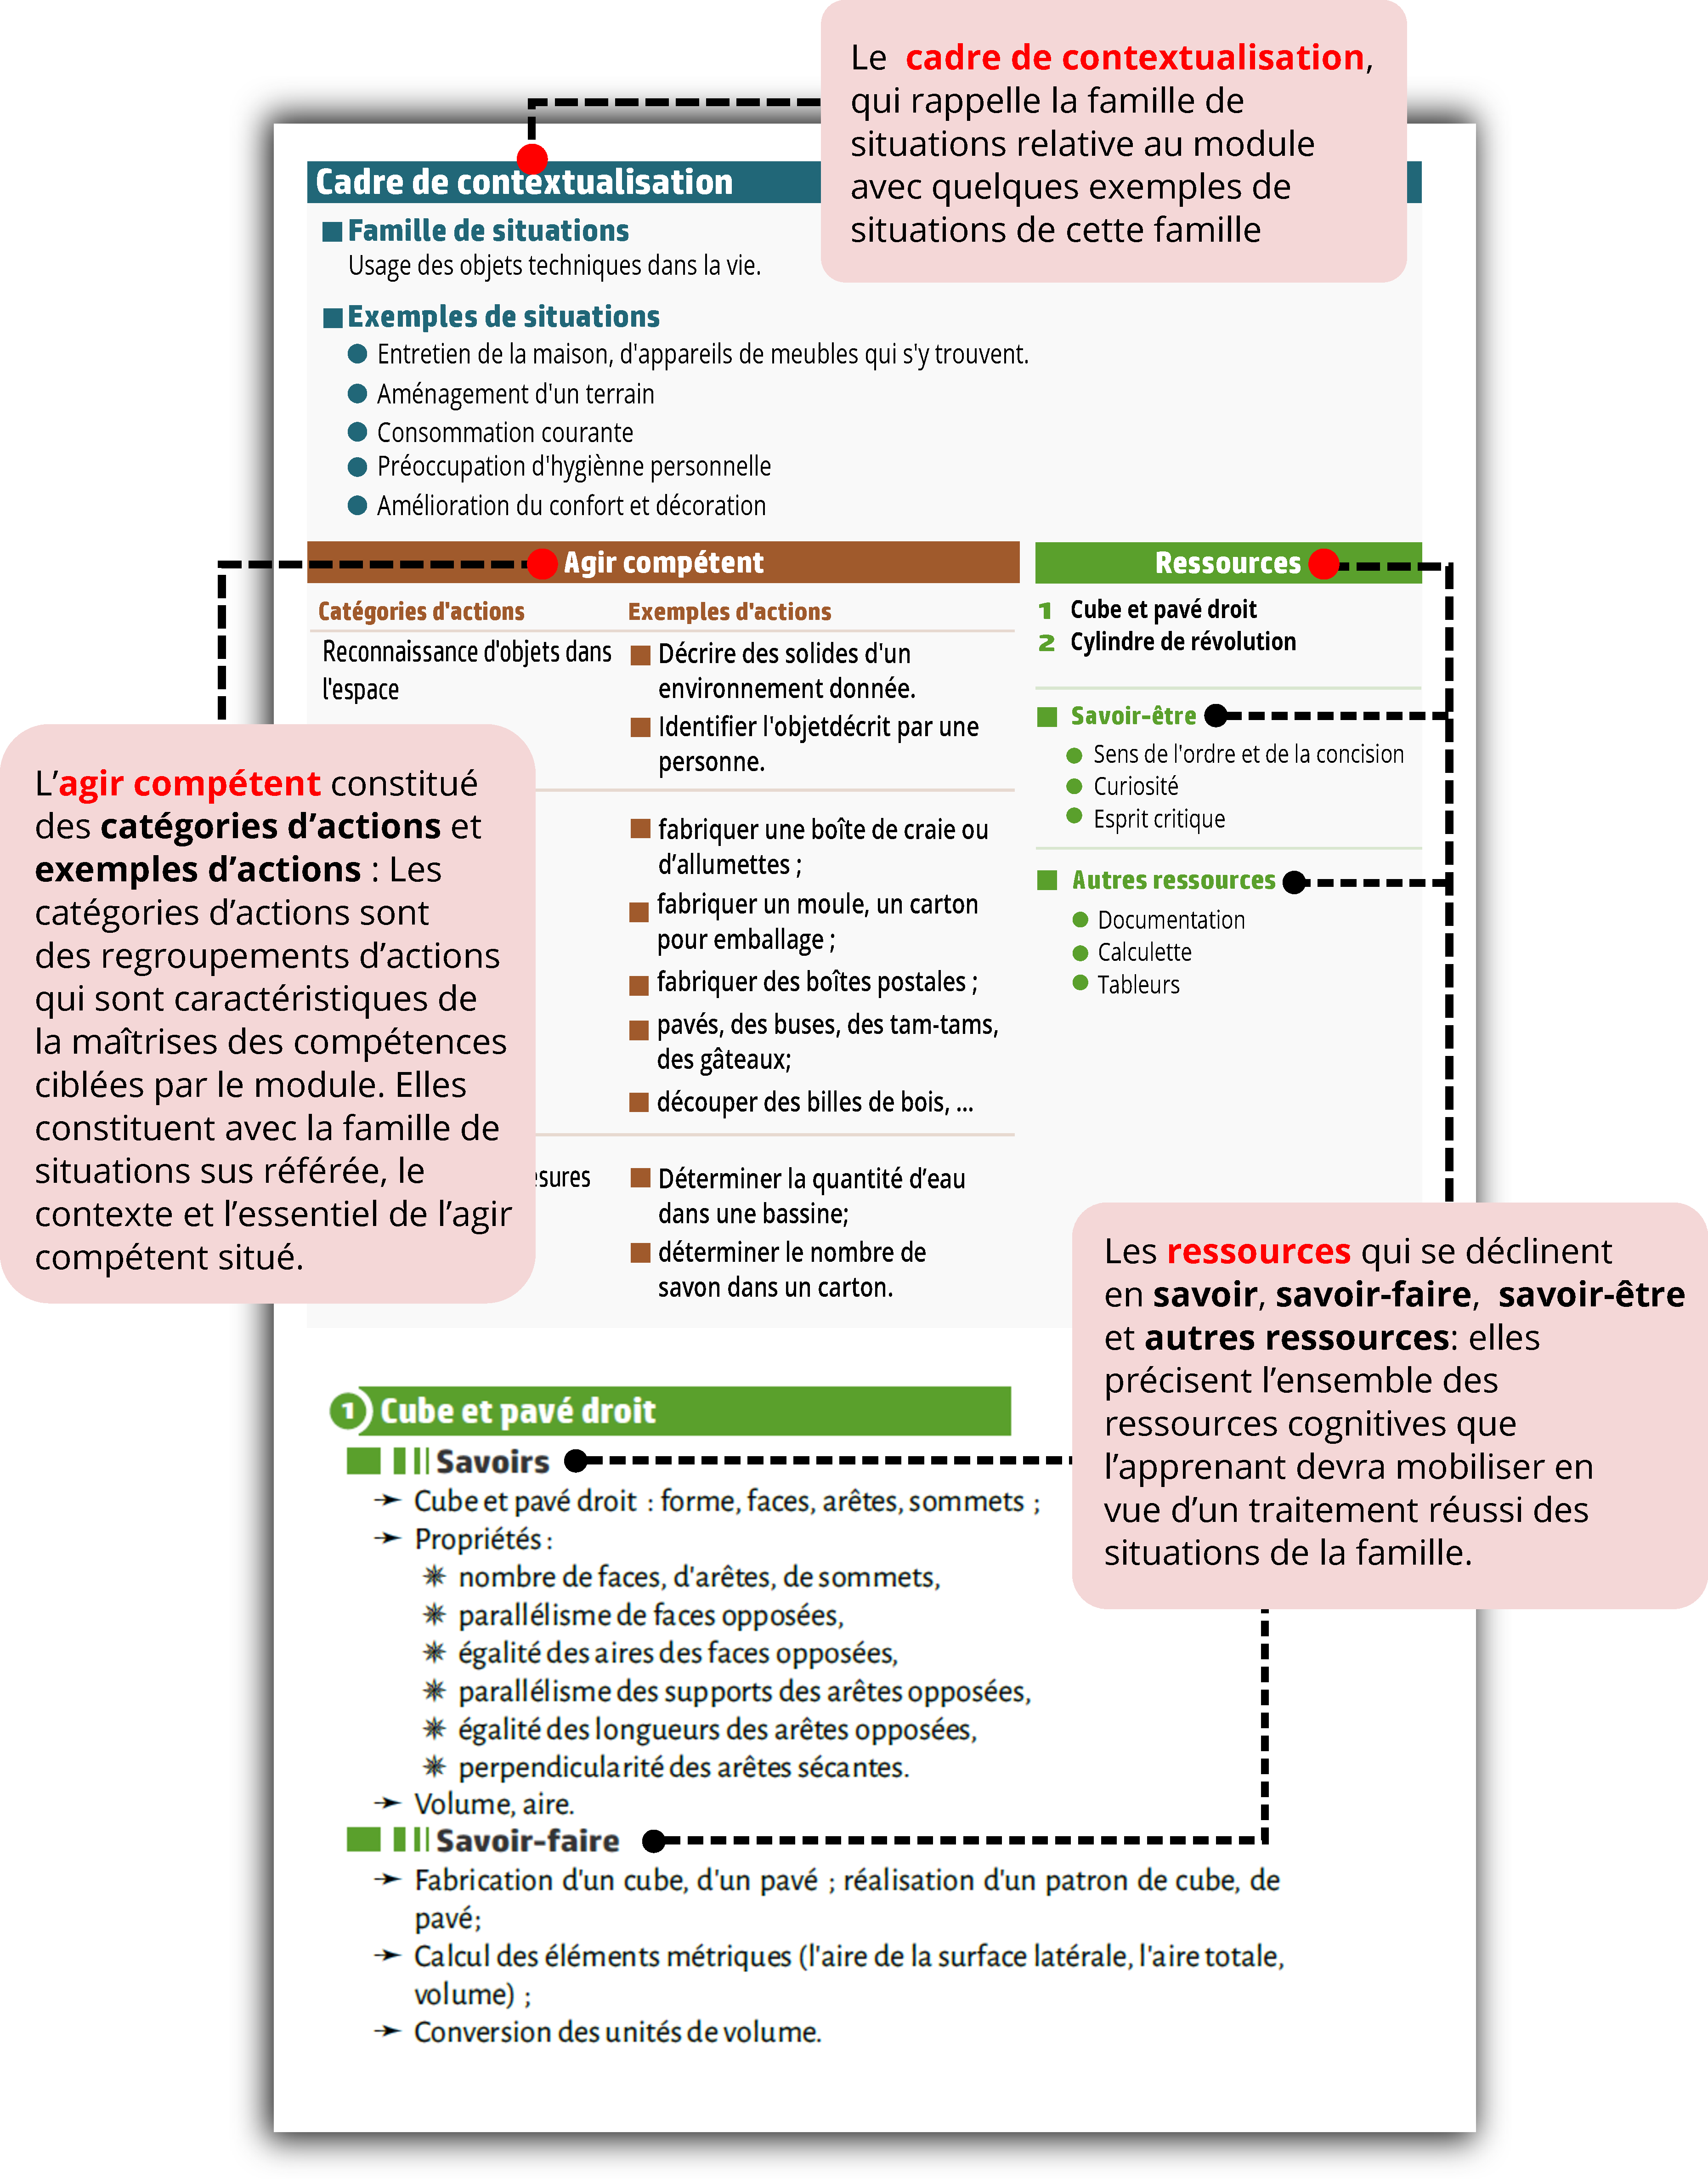
\includegraphics[width=\textwidth]{Pres.pdf}
\end{center}

\section*{Quelques recommandations d'ordre pédagogiques}
\addcontentsline{toc}{section}{Quelques recommandations d'ordre pédagogiques}
\subsection*{Méthodologie recommandée}
\addcontentsline{toc}{subsection}{Méthodologie recommandée}

L'approche par les compétences se fonde sur une pédagogie socio constructiviste. L'appropriation des savoirs mathématiques et le développement des compétences ne se transmettent pas, ils se construisent. Il importe pour cela, d'opter résolument pour une approche privilégiant l'activité de l'élève.\\
Dans cette perspective, les leçons de mathématiques doivent être basées sur des activités d'apprentissage et leur conduite doit être centrée sur l'apprenant. Aussi, chaque séquence d'enseignement/ apprentissage peut s'articuler autour des points suivants :
\begin{itemize}
\item Une introduction destinée à captiver l'attention des élèves et à contrôler les prérequis nécessaires ;
\item Une ou deux activités d'apprentissage destinées à favoriser l'acquisition des savoirs nouveaux ou à consolider des acquis antérieurs par les élèves eux-mêmes ;
\item L'essentiel à retenir en termes de notions ou de méthodes ;
\item Des exercices d'application ;
\item Des activités d'intégration si possible tant il est vrai qu'elles ont pour fonction d'amener les élèves à s'exercer sur la mobilisation de plusieurs acquis pour résoudre des problèmes courants. Elles peuvent se situer au terme de plusieurs apprentissages qui forment un tout significatif.
\item Il importe de préciser que les séances d'exercices sont des moments d'apprentissage à part entière. Elles doivent aussi être conduites de façon active.
\item Il importe aussi de comprendre que l'efficacité des actions entreprises pour rendre les élèves compétents ne s'accommode pas de la navigation à vue. L'élaboration des projets pédagogiques est de ce point de vue, une nécessité.
\end{itemize}

\subsection*{Evaluation}
\addcontentsline{toc}{subsection}{Evaluation}

Chaque épreuve écrite de contrôle des apprentissages devra tenir compte de l'évaluation des savoirs mathématiques et de l'évaluation des compétences, le tout encastré dans une charpente ayant les deux parties suivantes :
\begin{enumerate}
\item  \textbf{Travaux numériques }: Il s'agit par exemple d'évaluer la capacité à pratiquer le calcul exact, approché ou littéral ; à gérer des situations de vie par lecture/construction des tableaux ou par identification/résolution des modèles mathématiques sous-jacents ….
\item \textbf{Travaux géométriques} : Ils peuvent évaluer la capacité à représenter des objets usuels du plan, à décrire ou à caractériser des solides de l'espace, à calculer des grandeurs rattachées à ces objets, à gérer des situations de vie par l'utilisation de ces objets, …
\end{enumerate}
Les évaluations orales pendant les séances de classe sont encouragées. Elles permettent d'évaluer chez les élèves la capacité à communiquer en langage mathématique qui est l'une des compétences fondamentales de cette discipline ; elles constituent aussi, une source de motivation pour les élèves.\\
Les niveaux d'exigence ne doivent pas excéder le troisième niveau de la\textit{ taxonomie de BLOOM}. Ils doivent alors se limiter à la connaissance, la compréhension ou l'application (relativement simple).

\subsection*{Quelques consignes relatives aux contenus et aux apprentissages}
\addcontentsline{toc}{subsection}{Quelques consignes relatives aux contenus et aux apprentissages}
\subsubsection*{Langage ensembliste}
\addcontentsline{toc}{subsubsection}{Langage ensembliste}
Le professeur introduira, progressivement et à chaque fois que cela sera nécessaire, les notions et symboles ensemblistes $\emptyset, \in, \notin, \subset, \cup$ et $\cap$.\\
Il ne saurait être question de traiter la théorie des ensembles pour elle-même. De même, on introduira les notations des ensembles de nombres :  $\G N, \G Z$ et $\G D$ sans pour autant faire de leçon spécifique sur chaque ensemble.
\subsubsection*{Comparaison des nombres}
\addcontentsline{toc}{subsubsection}{Comparaison des nombres}
On habituera, tout au long du cycle, les élèves à utiliser un support graphique pour visualiser des notions numériques (comparaison, encadrement).
\subsubsection*{Calculatrices}
\addcontentsline{toc}{subsubsection}{Calculatrices}
La calculatrice est un outil qui, avec ou sans instructions officielles, connaît une large diffusion. Il est de l'intérêt des enseignants d'en tenir compte. S'il ne peut
être question, vu les coûts, d'imposer son usage par des mentions dans les programmes officiels, il importe de recenser à tous les niveaux les points de programmes et les
activités motivant son emploi et favorisant chez l'élève l'habitude d'une utilisation intelligente.
\subsubsection*{Apprentissage de la rigueur et abus de langage}
\addcontentsline{toc}{subsubsection}{Apprentissage de la rigueur et abus de langage}
Le professeur conduira progressivement les élèves au niveau de rigueur de langage souhaitable, mais tolérera les abus consistant à confondre par exemple
longueur et mesure. On ne se privera pas d'utiliser des formulations habituelles telles que :"\textit{La longueur du segment est 5 cm}" ou "\textit{un segment de 5 cm}", "\textit{Une surface de 3 cm$²$} ", "L\textit{e volume du prisme est de 4 l} ","\textit{Un angle de 30$^{\circ}$} ".
\subsubsection*{Angles}
\addcontentsline{toc}{subsubsection}{Angle}
Les notions d'angle et de secteur angulaire sont des notions difficiles à mettre en place de façon rigoureuse. Préférence sera donnée à être en accord avec le langage courant.
\subsubsection*{Espace}
\addcontentsline{toc}{subsubsection}{Espace}
L'étude de l'espace est répartie sur la totalité du cursus. Le problème de la représentation plane de configurations de l'espace se pose ; cette représentation ne
peut pas suppléer l'observation effective et, si possible, la construction des solides sera effectuée par les élèves.
\subsubsection*{Configurations planes}
\addcontentsline{toc}{subsubsection}{Configurations planes}
On s'efforcera de présenter des configurations planes que l'élève peut rencontrer hors de l'école ou qu'il peut réemployer (exemples de polygones réguliers en
classe de 5ème pour pouvoir proposer ultérieurement des exemples de prisme droit à base régulière). Mais, il ne peut être question de leur donner la même place qu'aux
configurations fondamentales, outils de raisonnement couramment employés; on demandera à l'élève de justifier, par exemple, qu'un triangle est équilatéral; on se
contentera, par contre, de lui demander de reconnaître un hexagone. On n'oubliera pas de proposer aux élèves des cas de figures trop souvent délaissés (exemple :
triangle avec un angle obtus pour la recherche des hauteurs et de l'orthocentre).
\subsubsection{Gestion des modules}
\addcontentsline{toc}{subsubsection}{Gestion des modules}
Dans l'ensemble un module forme un tout cohérent, mais il ne serait pas pertinent de terminer un module avant de commencer le suivant ; nous conseillons donc
au professeur d'alterner les activités numériques et les activités géométriques : par exemple on pourra étudier de front les modules 1 et 3, 2 et 4 pour la classe de sixième
et les modules 5 et 7, 6 et 8 pour la classe de cinquième.

%\newcounter{module}
%\setcounter{module}{1}
%\renewcommand{\thechapter}{\themodule}

\part*{Classe de sixième}
\addcontentsline{toc}{part}{Classe de sixième}

\setcounter{chapter}{0}
\renewcommand{\chaptername}{Module}

\chapter{Relations et opérations fondamentales dans l'ensemble des nombres décimaux et des fractions}
%\stepcounter{module}
 
{\AlegreyaSansLight \large
\begin{center}
\textbf{Crédit :} 32 heures\\
\textit{4 heures hebdomadaires}
\end{center}
}

\minitoc

\section{Introduction}
\subsection{Présentation du module}
Ce module vise à rendre l'apprenant compétent dans des situations de vie de la famille « \textit{représentation, détermination des quantités et identification des objets
par des nombres} ». Il s'agit en gros, de le rendre capable de :
\begin{itemize}
\item Résoudre des problèmes relatifs à des situations de vie telles que : l'achat ou la vente des biens de consommation, le partage des biens, la vérification
d'une facture après payement, la comparaison des prix des objets …
\item Communiquer des informations comportant des nombres (numéros de téléphones, matricule, immatriculation d'un véhicule …).
\end{itemize}
Il importe pour cela de consolider les notions d'addition, de soustraction, de multiplication, de division et de relation d'ordre vues dans le cycle primaire avec
cependant une démarcation significative dans l'introduction et la manipulation des nombres décimaux relatifs, sur lesquels l'utilisateur devrait s'appesantir un peu plus.
On restera au niveau des habiletés cognitives que sont : la connaissance et la compréhension.\\
En dehors de la maîtrise des techniques opératoires, il est question de donner du sens aux nombres décimaux et de les utiliser dans des situations de vie qui l'exigent.

\subsection{Contribution du module à la finalité et aux buts curriculaires}
Ce module permet de développer le sens de l'ordre, de la concision et l'esprit critique. Il contribue au renforcement de la pratique du calcul mental ou à l'utilisation de la calculatrice, ce qui permet à l'apprenant d'agir de manière autonome, compétente et adaptative dans diverses situations de la vie courante, dans lesquelles ces pratiques interviennent.

\subsection{Contribution du module au programme d'études et aux domaines de vie}
Ce module qui fait partie des programmes de mathématiques permet à chaque apprenant d'acquérir des connaissances et savoir-faire de base sur lesquels les
enseignements/apprentissages qu'il recevra ultérieurement dans les autres disciplines du domaine d'apprentissage devront s'appuyer. Les nombres décimaux sont
utilisés dans toutes les sciences pour mesurer, peser et évaluer les quantités.\\
La maîtrise des concepts d'égalité, d'inégalité et des opérations fondamentales que sont l'addition, la soustraction, la multiplication et la division, est de nature à
doter l'apprenant d'un des outils fondamentaux dont il aura besoin tout au long de sa vie. La gestion du budget familial, la comptabilité au sein de l'entreprise,
l'évaluation des distances, des poids, des aires et des volumes, sont autant d'applications des nombres décimaux dans les domaines de vie que sont l'économie, les
média, l'environnement, la santé et le bien être.

\section{Matrice}


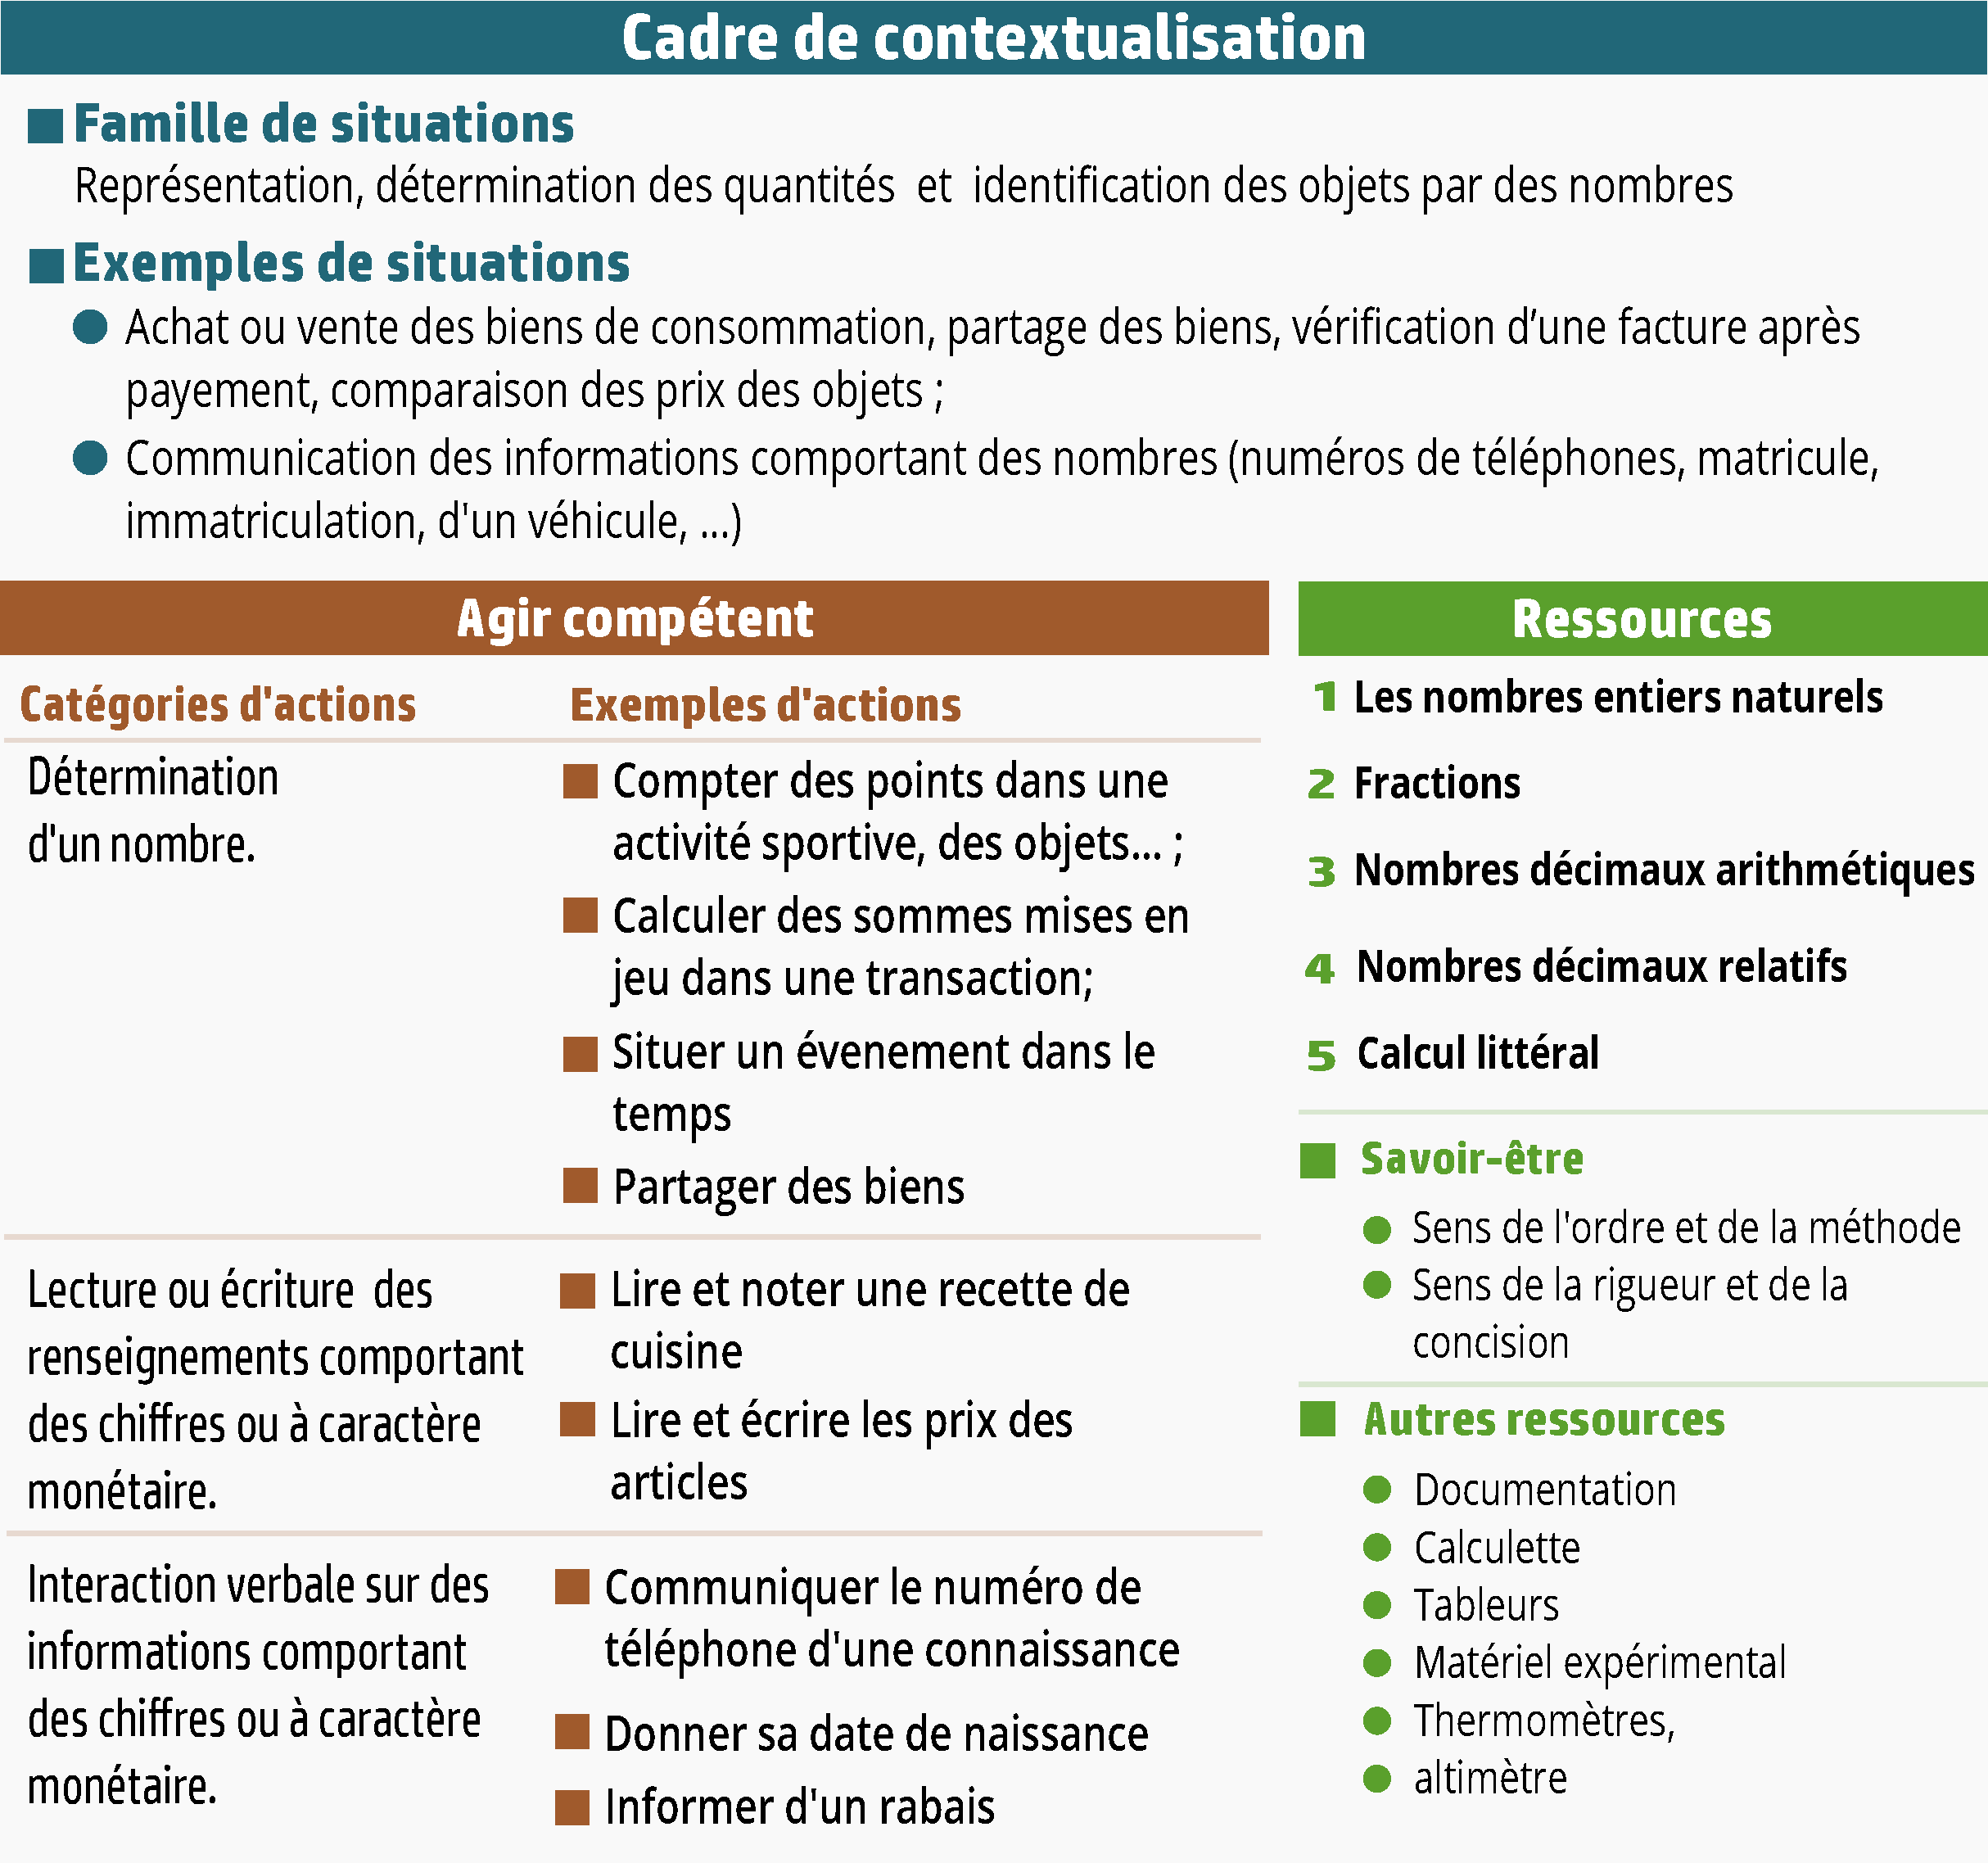
\includegraphics[width=\textwidth]{Module1.pdf} 

\subsection*{}
\addcontentsline{toc}{subsection}{\textbf{Ressource 1}: Les nombres entiers naturels}
\ressource{IN.pdf}

\savoir
\begin{itemize}
\item Multiples et diviseurs d'un entier naturel.
\item Entiers naturels et ordre ;
\item Entiers naturels consécutifs ;
\item Propriétés d'addition et de multiplication des nombres entiers naturels.
\end{itemize}
\savoirfaire
\begin{itemize}
\item Lecture et écriture des entiers;
\item Opérations d'addition, de soustraction, de multiplication et de division;
\item Division à l'aide des critères de divisibilité : par 10, 100, 1000, .., par 2 , 3, 5 et  9;
\item Nombre d'entiers consécutifs de m à n où n et m sont des entiers naturels.
\end{itemize}

\subsection*{}
\addcontentsline{toc}{subsection}{\textbf{Ressource 2}: Les fractions}
\ressource{Fractions.pdf}

\savoir
\begin{itemize}
\item Numérateur, dénominateur, fractions égales, fractions irréductibles, fractions décimales ;
\item Inverse d'une fraction;
\item Propriétés d'addition et de multiplication des fractions.
\end{itemize}
\savoirfaire
\begin{itemize}
\item Ecriture fractionnaire d'un nombre décimal;
\item Simplification des fractions;
\item Addition et soustraction des fractions de même dénominateur;
\item Multiplication, division des fractions;
\item Comparaison des fractions.
\end{itemize}

\subsection*{}
\addcontentsline{toc}{subsection}{\textbf{Ressource 3}: Nombres décimaux arithmétiques}
\ressource{ID.pdf}

\savoir
\begin{itemize}
\item Lecture et écriture d'un nombre décimal;
\item Propriétés d'addition et de multiplication des nombres décimaux.
\end{itemize}
\savoirfaire

\textbf{Techniques et méthodes}
\begin{itemize}
\item \textit{Opérations} : addition, soustraction, multiplication, division ;
\item Comparaison des nombres décimaux..
\end{itemize}

\subsection*{}
\addcontentsline{toc}{subsection}{\textbf{Ressource 4}: Nombres décimaux relatifs}
\ressource{Z.pdf}

\savoir
\begin{itemize}
\item Nombres entiers relatifs;
\item Opposé d'un nombre décimal relatif.
\end{itemize}
\savoirfaire
\begin{itemize}
\item Somme d'entiers relatifs;
\item Somme de décimaux relatifs.
\end{itemize}

\subsection*{}
\addcontentsline{toc}{subsection}{\textbf{Ressource 5}: Calcul littéral}
\ressource{CL.pdf}

\savoir

\textbf{Règles de priorité des opérations :}
\begin{itemize}
\item opérations avec parenthèses ;
\item opérations sans parenthèses ;
\item suite de multiplications et de divisions sans parenthèses.
\end{itemize}
\savoirfaire
\begin{itemize}
\item Valeur numérique d'une expression littérale simple ;
\item Utilisation des propriétés de l'addition et de la multiplication des nombres décimaux positifs ;
\item Calcul rapide
\end{itemize}
\chapter{Organisation et gestion des données}
%\stepcounter{module}

{\AlegreyaSansLight \large
\begin{center}
\textbf{Crédit :} 11 heures\\
\textit{4 heures hebdomadaires}
\end{center}
}

\minitoc

\section{Introduction}

\subsection{Présentation du module}
Ce module vise à rendre l'apprenant capable de traiter de façon réussie, des situations de vie de la famille  "organisation des données et estimation des quantités dans la consommation des biens et services ". Il s'agit pour lui de :
\begin{itemize}
\item Déployer un raisonnement mathématique pour identifier et formaliser des situations de vie qui se rapportent aux proportionnalités.
\item Résoudre des problèmes relatifs à des situations telles que le placement d'argent, la remise au cours d'achat divers, le partage proportionnel.
\end{itemize}
Pour y parvenir, il est nécessaire de consolider et de renforcer les acquis sur les proportionnalités, les pourcentages et l'échelle vue au cycle primaire tout en restant sur les habiletés cognitives que sont la connaissance, la compréhension et l'application.\\
Ce module est par excellence celui qui, à ce niveau d'étude, comporte les situations de vie les plus familières à l'élève.

\subsection{Contribution du module à la finalité et aux buts curriculaires}
Le module permet de développer les compétences transversales suivantes : le sens de la concision, l'esprit critique et l'organisation rationnelle des données. A terme, ces compétences permettent à l'apprenant de s'assumer comme membre responsable d'une famille, en même temps qu'elles lui permettent d'opérer des choix
judicieux et autonomes, dans la production, la consommation des biens et services.

\subsection{Contribution du module au programme d'études et aux domaines de vie}
Ce module est un des maillons essentiels du programme de 6ème et de 5ème. Il est par excellence l'exemple d'intégration des mathématiques dans la vie quotidienne. Les situations de vie et les exemples d'actions auxquelles il renvoie, de même que toutes les autres composantes du module pourront tout aussi bien intervenir en physique, dans les sciences de la vie et de la terre, en géographie, et plus tard en psychologie et en économie, et surtout dans les situations de vie. Il permet à ce niveau de dégager de manière implicite et même transversale l'importance de l'interdisciplinarité dans plus d'un domaine d'apprentissage.\\
La maîtrise de ces deux notions que ce module développe est de nature à doter l'apprenant d'outils essentiels dont il a besoin dans la vie pratique. Sa contribution dans la gestion du budget familiale est indéniable. Son implication dans la détermination des quantités justifie son importance dans la consommation des biens. Une bonne maîtrise des pourcentages situés (utilisés dans une situation de vie) est un atout majeur dans la consommation des informations, et dans l'exploitation, l'analyse et l'interprétation des données à caractère économique ou social.

\section{Matrice}

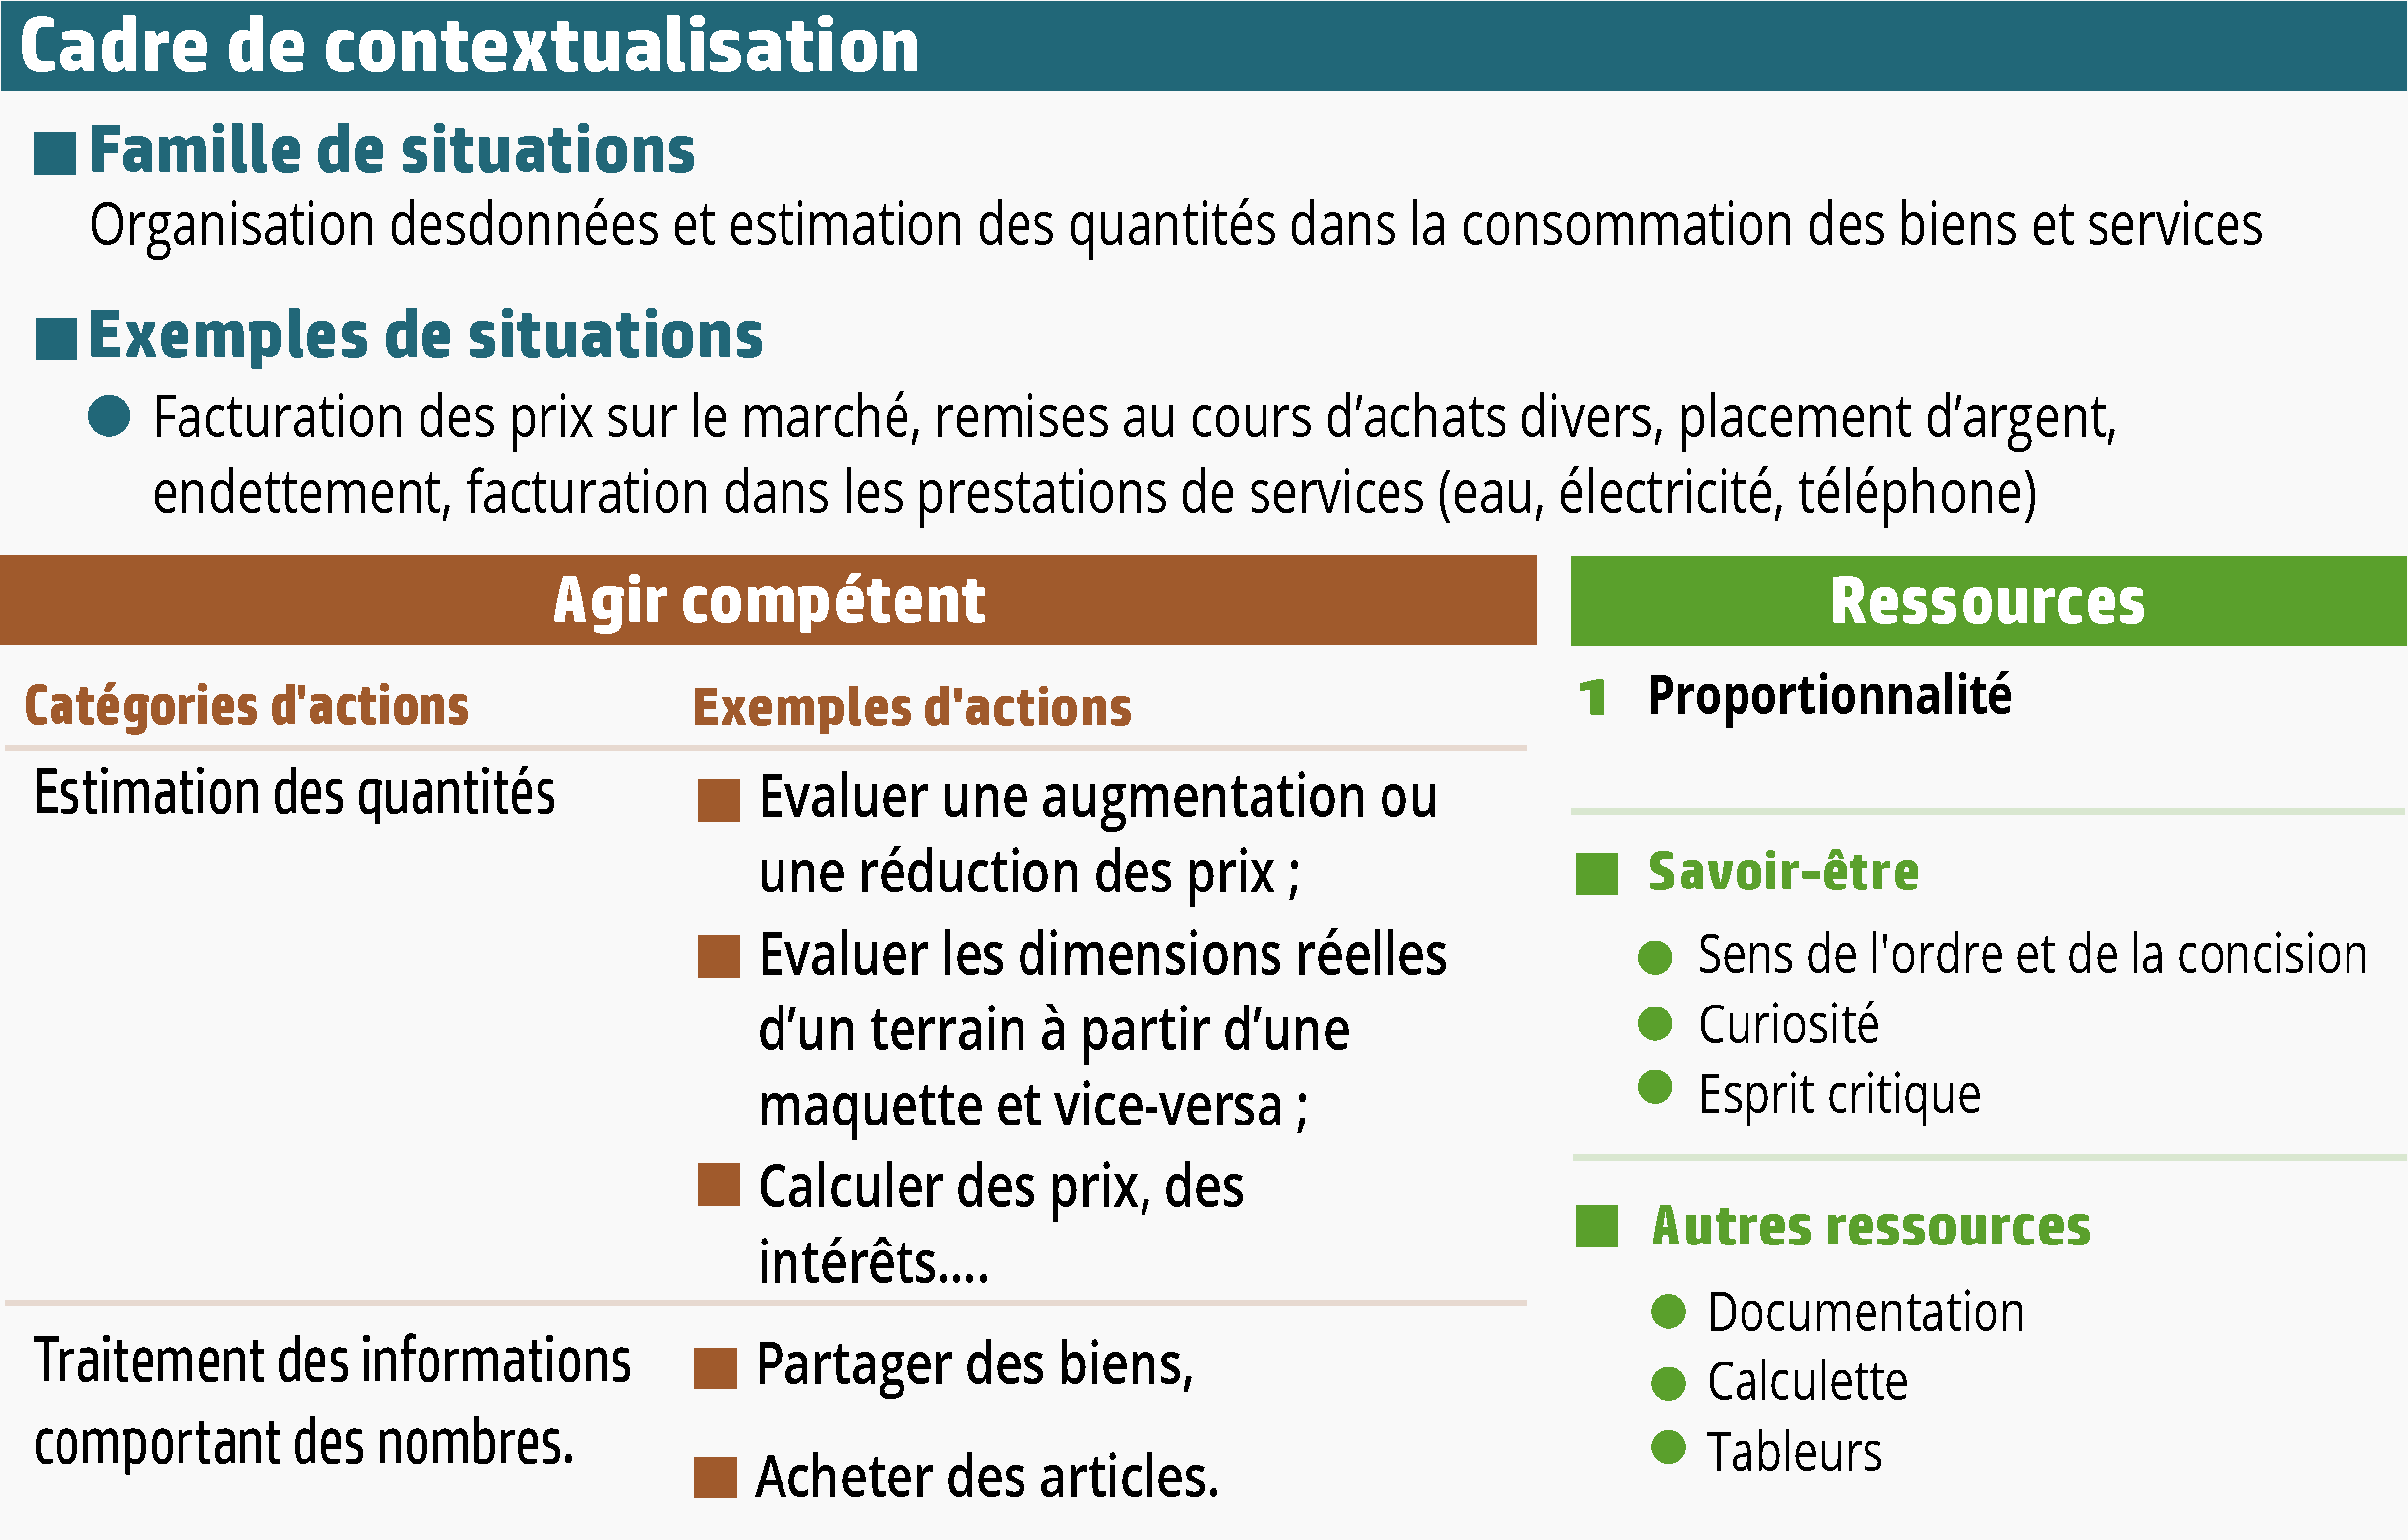
\includegraphics[width=\textwidth]{Module2.pdf} 

\subsection*{}
\addcontentsline{toc}{subsection}{\textbf{Ressource}: proportionnalité}
\ressource{Prop.pdf}

\savoir
\begin{itemize}
\item Tableau de proportionnalité ;
\item Coefficients de proportionnalité ;
\item Suite de nombres proportionnels ;
\item Quatrième proportionnelle ;
\item Pourcentage, échelle ;
\item Propriétés des nombres proportionnels.
\end{itemize}
\savoirfaire
\begin{itemize}
\item Utilisation des coefficients de proportionnalités comme opérateurs ;
\item Utilisation des propriétés des nombres proportionnels pour déterminer des quantités ;
\item Utilisation des pourcentages et des échelles comme opérateurs.
\end{itemize}
\chapter{Configurations et transformations élémentaires du plan}
%\stepcounter{module}

{\AlegreyaSansLight \large
\begin{center}
\textbf{Crédit :} 46 heures\\
\textit{4 heures hebdomadaires}
\end{center}
}

\minitoc

\section{Introduction}

\subsection{Présentation du module}
Ce module comporte deux parties essentielles : les configurations planes, les symétries orthogonales et centrales dans le plan. Il développe deux compétences fondamentales que sont :
\begin{itemize}
\item déployer un raisonnement mathématique du type analogique, déductif et inductif ;
\item résoudre des problèmes par l'observation, l'identification et la caractérisation des formes planes ; par les transformations élémentaires que sont les symétries.
\end{itemize}
Il s'articule sur la famille de situations suivantes : représentations et transformations des configurations planes dans l'environnement. Les compétences mises en contexte s'appuient sur les trois catégories d'actions qui suivent :
\begin{itemize}
\item Reconnaissance des formes planes et des transformations dans l'environnement physique ;
\item Production des formes planes et transformations dans l'environnement physique ;
\item Détermination des mesures et des positions
\end{itemize}
Cette dernière catégorie d'actions est le champ privilégié de l'inter action entre les activités numériques et les activités géométriques de l'élève de 6ème.\\
Les différentes actions qui s'intègrent dans chacune des catégories suscitées sont en corrélation avec les savoirs essentiels que ce module développe, et qui s'appuient sur les habiletés cognitives suivantes : connaissance, compréhension et application.
\subsection{Contribution du module à la finalité et aux buts curriculaires}
A travers les différents raisonnements sus évoqués, l'apprenant développe les compétences transversales suivantes : le sens de l'ordre ; de la rigueur et de la concision ; le sens de l'initiative et de la créativité ; la pensée critique. Ils les développent en les intégrant, dans le cadre d'une démarche scientifique. Ces compétences contribuent à la formation d'un citoyen autonome et responsable dans l'exercice de ses rôles sociaux

\subsection{Contribution du module au programme d'études et aux domaines de vie}
La géométrie plane occupe une place privilégiée dans le programme de mathématiques de par les compétences qu'elle vise à développer. Sa contribution au développement de la technologie, de l'art, de la chimie, ne sont plus à démontrer. Enfin les innombrables symétries que la nature offre dans la biologie et la physiologie végétale ou animale font de ce module un des maillons essentiels dans plus d'un domaine d'apprentissage.\\
L'importance de ce module réside dans le fait que l'élève vit dans un espace géographique. L'utilisation et la rencontre des objets dans lesquels on peut extraire des formes géométriques planes font partie du quotidien : aménagement ou réalisation de son habitat, manipulation ou réalisation de certains objets usuels , appréciation ou production des œuvres d'art, choix du chemin adéquat pour se rendre à un lieu pour ne citer que celles-ci ; toutes choses pouvant l'aider à s'affirmer comme membre responsable d'une famille, à opérer des choix judicieux dans la consommation des biens , des services et de l'information. La contribution de ce module à tous les domaines de vie est donc d'une évidence incontestable.

\section{Matrice}

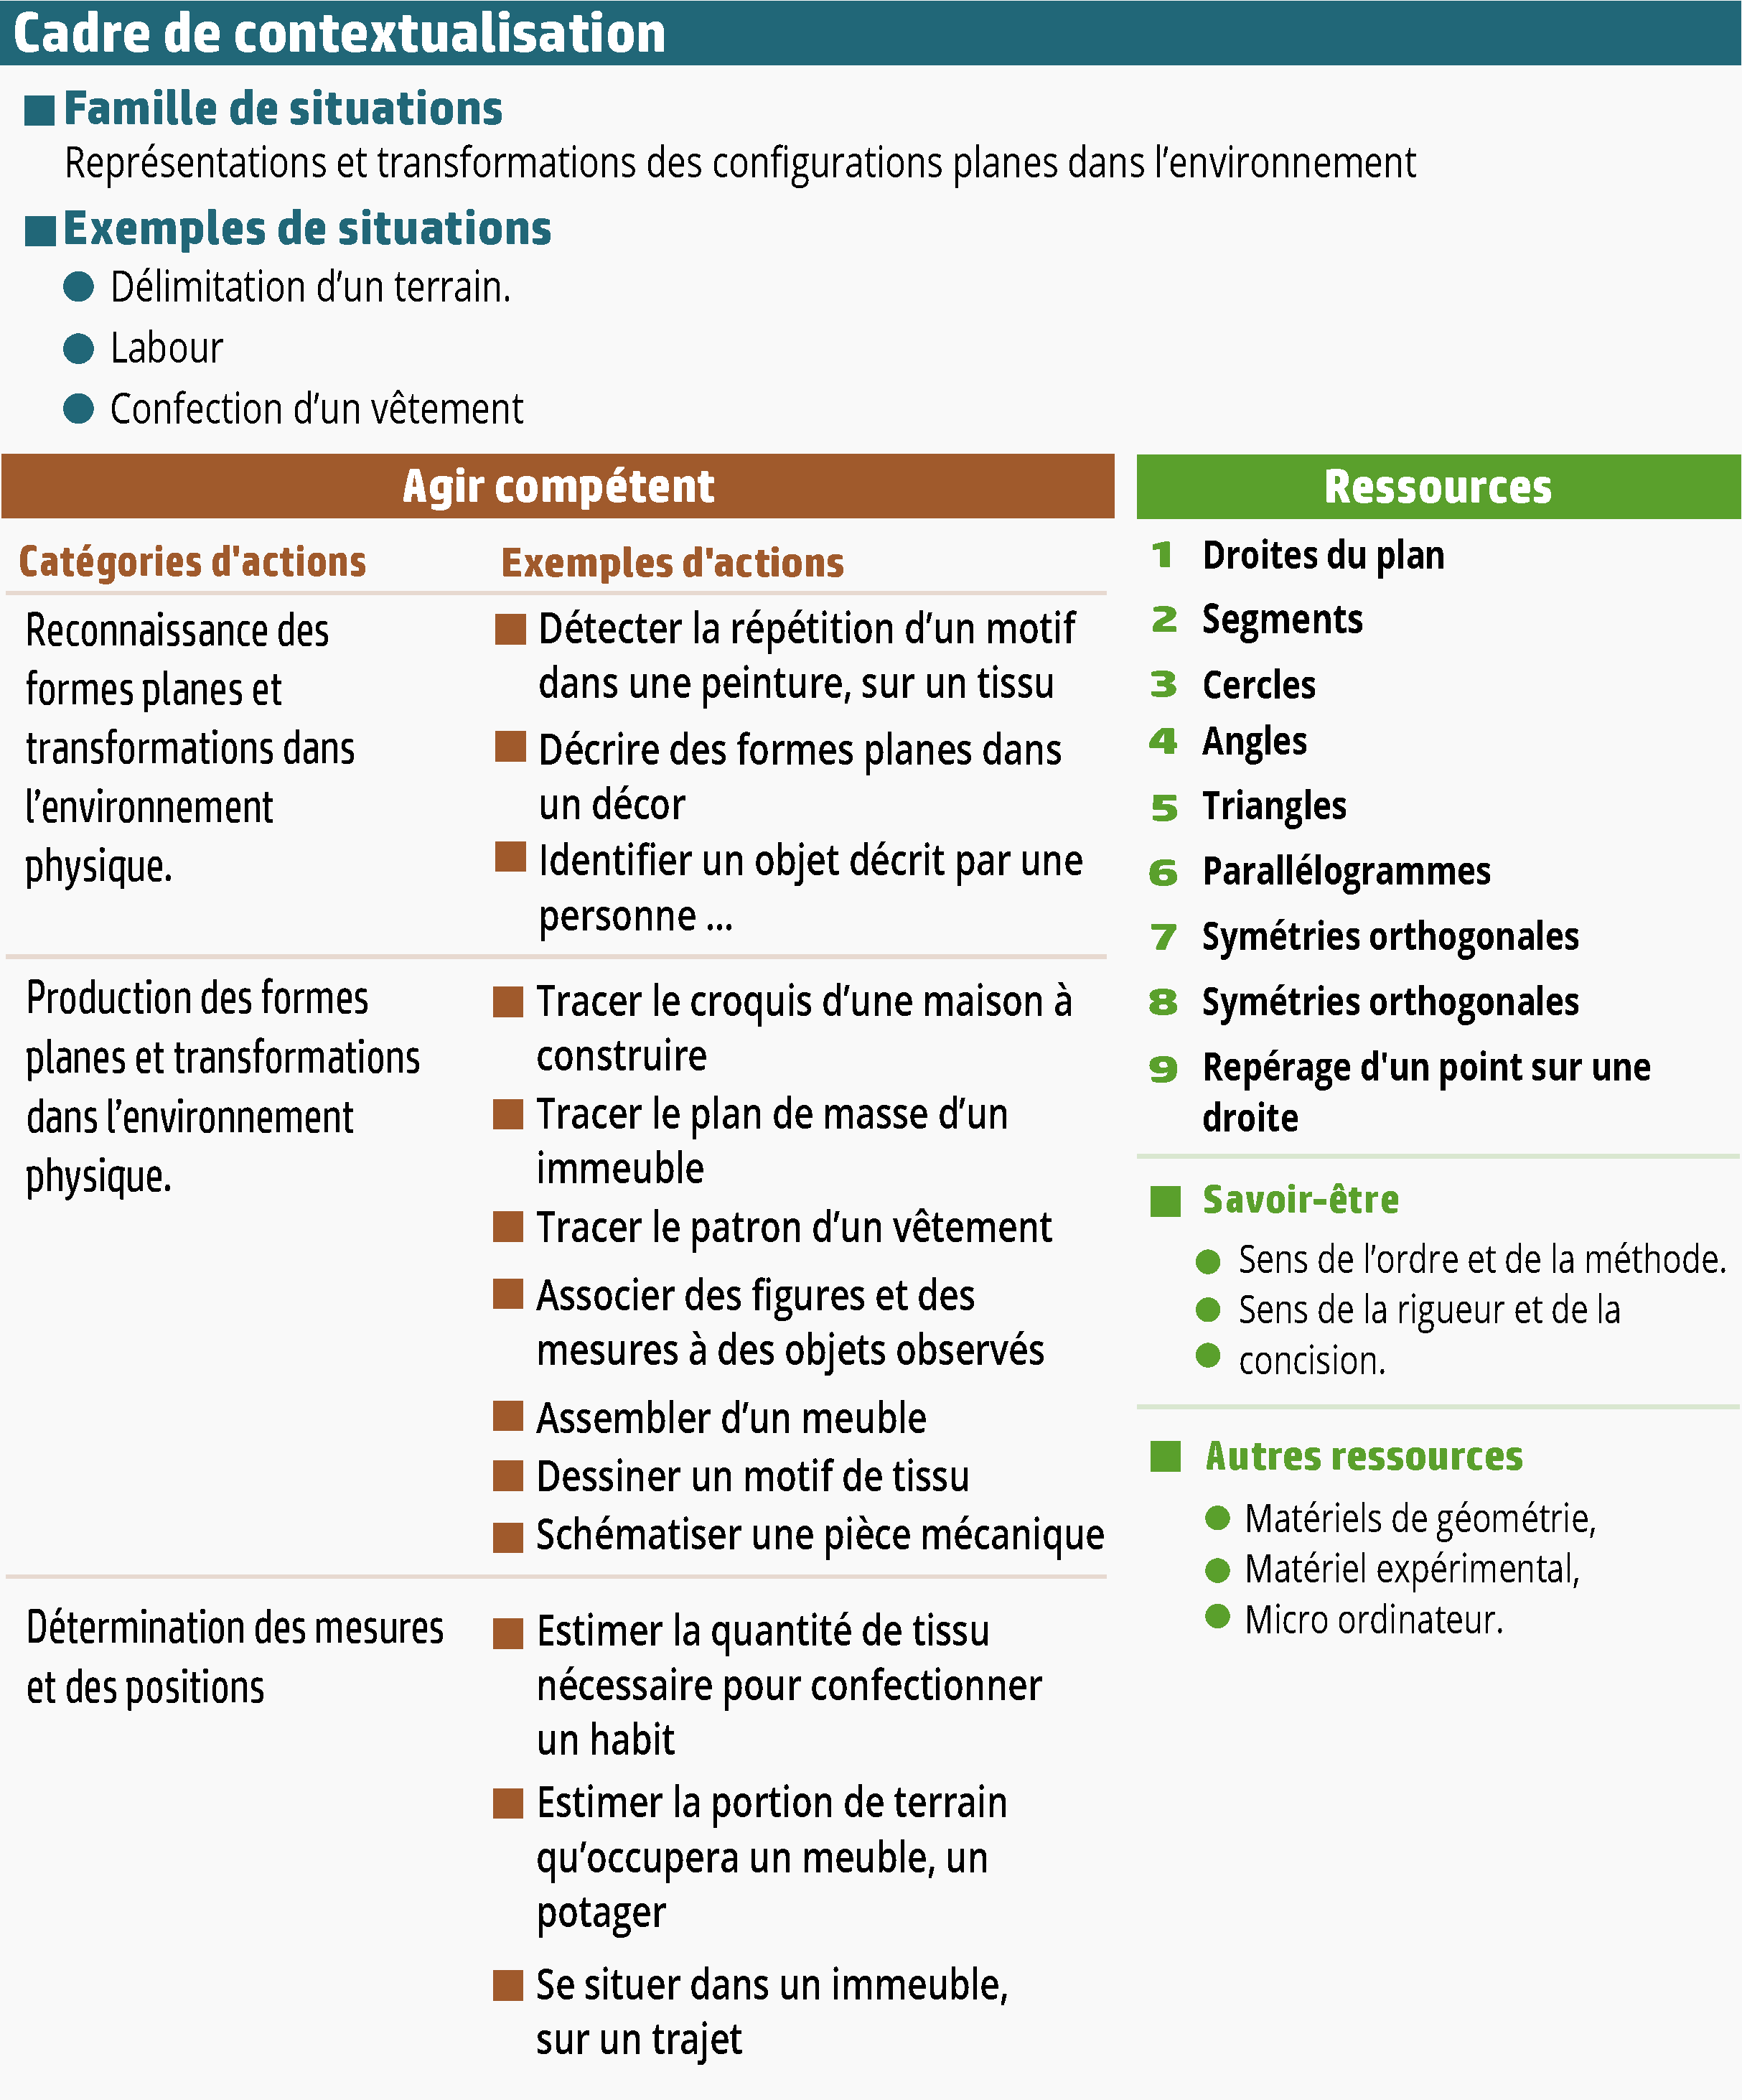
\includegraphics[scale=.36]{Module3.pdf} 

\subsection*{}
\addcontentsline{toc}{subsection}{\textbf{Ressource 1}: droites du plan}
\ressource{DP.pdf}

\savoir
\begin{itemize}
\item Droites : appartenance de points, notation, points alignés ;
\item Droites passant par :
\begin{itemize}
\item un point,
\item deux points distincts.
\end{itemize}
\item Régionnement du plan par une droite ;
\item Quatrième proportionnelle ;
\item Demi-droites ;
\item Droites sécantes;
\item Droites perpendiculaires :
\begin{itemize}
\item Symbolisme ;
\item \textit{Par un point donné, il passe une et une seule perpendiculaire à une droite donnée.}
\end{itemize}
\item Droites parallèles :
\begin{itemize}
\item Symbolisme ;
\item\textit{ Par un point donné, il passe une et une seule parallèle à une droite donnée ;}
\item \textit{Lorsque deux droites sont parallèles, toute parallèle (sécante, perpendiculaire)
à l'une est parallèle (sécante, perpendiculaire) à l'autre ;}
\item \textit{Deux droites perpendiculaires à une même droite sont parallèles.}
\end{itemize}
\end{itemize}
\savoirfaire
\begin{itemize}
\item Construction à l'aide des instruments (règle et équerre) :
Droite passant par 2 points, droite passant par un point et parallèle à une autre, droite passant un point et perpendiculaire à une autre.
\end{itemize}

\subsection*{}
\addcontentsline{toc}{subsection}{\textbf{Ressource 2}: segments}
\ressource{Seg.pdf}

\savoir
\begin{itemize}
\item Segments, support d'un segment ;
\item Longueur d'un segment ;\\
\textit{Propriété} : Si  $M\in\ife{AB}$ alors $MA+MB=AB$.
\item Milieu d'un segment ;\\
\textit{Propriété} : Si M est milieu du segment $\ife{AB}$ alors $MA=\dfrac{AB}{2}=MB$
\item Médiatrice d'un segment: définition.
\end{itemize}
\savoirfaire
\begin{itemize}
\item Construction de la médiatrice d'un segment à l'aide de la règle et de l'équerre ;
\item Construction d'un segment donné ;
\item Construction du milieu d'un segment donné à l'aide de la règle graduée;
\item Conversion des unités de longueur.
\end{itemize}

\newpage

\subsection*{}
\addcontentsline{toc}{subsection}{\textbf{Ressource 3}: cercle}
\ressource{Cer.pdf}

\savoir
\begin{itemize}
\item Rayon, diamètre, corde, arc, périmètre ou circonférence du cercle, disque, aire du disque ;
\item Positions relatives de deux cercles.
\end{itemize}
\savoirfaire
\begin{itemize}
\item Tracer un cercle de centre donné et de rayon donné ; 
\item Tracer un cercle de diamètre donné;
\item Calculer des éléments métriques (périmètre, aire, rayon, diamètre).
\end{itemize}

\subsection*{}
\addcontentsline{toc}{subsection}{\textbf{Ressource 4}: angles}
\ressource{Ang.pdf}

\savoir
\begin{itemize}
\item Notions d'angle et / ou de
secteur angulaire ;
\item \textit{Vocabulaire et notation}: sommet, côtés, angle saillant, nul, aigu, droit, obtus, plat, rentrant, plein ;
\item Mesures (en degrés) ;
\item Bissectrice.
\end{itemize}
\savoirfaire
\begin{itemize}
\item Construction d'un angle de mesure donnée ( à l'aide du rapporteur et de la règle) ;
\item Détermination de la mesure d'un angle donné ;
\item Construction de la bissectrice d'un angle donné à l'aide du rapporteur et de la règle. diamètre).
\end{itemize}

\subsection*{}
\addcontentsline{toc}{subsection}{\textbf{Ressource 5}: triangles}
\ressource{Tri.pdf}

\savoir
\begin{itemize}
\item Vocabulaire ;
\item Triangles particuliers ;
\item \textit{Droites particulières d'un triangle} : hauteur, médiane, bissectrice, médiatrice d'un côté ;
\item Périmètre et aire.
\end{itemize}
\savoirfaire
\begin{itemize}
\item Construction d'un triangle connaissant : les longueurs des côtés, la longueur de deux côtés et la mesure de l'angle qu'ils forment, la
longueur d'un côté et les mesures des angles à ses extrémités ;
\item Construction des triangles particuliers ;
\item Construction d'une hauteur, d'une médiane, d'une médiatrice, d'une bissectrice dans un triangle.
\item  Calcul du périmètre et de l'aire.
\end{itemize}

\subsection*{}
\addcontentsline{toc}{subsection}{\textbf{Ressource 6}: parallélogrammes}
\ressource{Par.pdf}

\savoir
\begin{itemize}
\item Parallélogramme, losange, rectangle, carré, périmètre et aire ;
\item \textit{Propriétés}: longueur des côtés opposés, diagonales, angles aux sommets opposés.
\end{itemize}
\savoirfaire
\begin{itemize}
\item Construction à l'aide du compas, de la règle et de l'équerre : du 4ème sommet d'un parallélogramme, d'un losange, d'un rectangle, d'un carré ;
\item Calcul de l'aire d'un parallélogramme, d'un losange, d'un rectangle, d'un carré;
\item Utilisation des propriétés pour justifier/déterminer une égalité de longueur, de mesure d'angle ;
\item  Techniques de conversion des unités d'aires.
\end{itemize}

\subsection*{}
\addcontentsline{toc}{subsection}{\textbf{Ressource 7}: symétries orthogonales}
\ressource{Syo.pdf}

\savoir
\begin{itemize}
\item Points symétriques par rapport à une droite.
\item \textit{Propriétés}: conservation de l'alignement, des longueurs, des angles, des formes.
\end{itemize}
\savoirfaire
\begin{itemize}
\item Construction du symétrique d'un point, d'une figure usuelle (segment, triangle, cercle, quadrilatères) par rapport à une droite. ;
\item  Utilisation des propriétés pour :
\begin{itemize}
\item justifier une égalité de longueur, de mesure d'angle ; 
\item déterminer une longueur, une mesure d'angle.
\end{itemize}  
\end{itemize}

\subsection*{}
\addcontentsline{toc}{subsection}{\textbf{Ressource 8}: symétries centrales}
\ressource{Syc.pdf}

\savoir
\begin{itemize}
\item Points symétriques par rapport à un point.
\item Propriétés: conservation de l'alignement, des longueurs, des angles, des formes.
\end{itemize}
\savoirfaire
\begin{itemize}
\item Construction du symétrique d'un point, d'une figure usuelle (segment, triangle, cercle, quadrilatères) par rapport à un point. ;
\item  Utilisation des propriétés pour:
\begin{itemize}
\item justifier une égalité de longueur, de mesure d'angle ; 
\item déterminer une longueur, une mesure d'angle.
\end{itemize}  
\end{itemize}

\subsection*{}
\addcontentsline{toc}{subsection}{\textbf{Ressource 9}: repérage d'un point sur une droite}
\ressource{Rep.pdf}

\savoir
\begin{itemize}
\item Demi-droite graduée, droite graduée ;
\item Origine, unité, abscisse d'un point, abscisse du milieu d'un segment.
\end{itemize}
\savoirfaire
\begin{itemize}
\item Placement d'un point d'abscisse donnée.  
\end{itemize}
\chapter{Solides de l'espace}
%\stepcounter{module}

{\AlegreyaSansLight \large
\begin{center}
\textbf{Crédit :} 11 heures\\
\textit{4 heures hebdomadaires}
\end{center}
}

\minitoc

\section{Introduction}

\subsection{Présentation du module}
Ce module comporte deux parties essentielles : cube et pavés droits ; cylindre de révolution. Il développe deux compétences fondamentales que sont :
\begin{itemize}
\item déployer un raisonnement mathématique (analogique, inductif et déductif)
\item résoudre des problèmes par l'observation, l'identification et la caractérisation des objets de l'espace.
\end{itemize}
Il s'articule sur la famille de situations suivante : usage des objets techniques dans la vie. Les compétences mises en contexte s'appuient sur les trois catégories d'actions qui suivent :
\begin{itemize}
\item Reconnaissance des solides dans l'espace.
\item Production d'objets.
\item Détermination des mesures.
\end{itemize}
Cette dernière catégorie d'actions est le champ privilégié de l'inter action entre les activités numériques et les activités géométriques de l'élève de 6ème.\\
Les différentes actions qui s'intègrent dans chacune des catégories suscitées sont en corrélation avec les savoirs essentiels que ce module développe, et qui s'appuient sur les habiletés cognitives suivantes : connaissance, compréhension et application.
\subsection{Contribution du module à la finalité et aux buts curriculaires}
L'apprentissage de la géométrie en général, et de la géométrie dans l'espace en particulier concourt à la construction du raisonnement, à la familiarisation avec les techniques calculatoires telles que les calculs d'aires et des volumes. Le traitement de la famille de situations aidera l'élève à construire ces éléments de formation. Il pourra également se familiariser avec les techniques de classement, d'observation et de description, de représentation, autant d'attitudes qui contribuent à l'autonomie.

\subsection{Contribution du module au programme d'études et aux domaines de vie}
Les éléments de formation que l'élève construira en traitant avec compétence la famille de situations choisie devrait l'aider à réaliser des actions et résoudre des problèmes.\\
De plus, le présent module est d'un apport significatif au domaine d'apprentissage intitulé « sciences et technologie », tant il participe à la conception, à la représentation, et à la réalisation des chefs d'œuvres architecturaux, et de tous les objets technologiques qui nous entourent. Sa contribution à la représentation de la structure cristalline de certains éléments de base en chimie mérite elle aussi d'être soulignée. Enfin il ne serait pas superflu de signaler sa contribution au développement du design, des arts plastiques et graphiques, véhicules de grandes valeurs universelles telles que l'esthétique et l'harmonie.\\
La contribution de ce module au développement de la technologie vient d'être soulignée plus haut. L'importance du développement de la technologie n'est plus
à démontrer dans la vie économique, et dans l'amélioration du bien être familial. On peut donc affirmer par voie de conséquence que la contribution de ce module à la vie sociale et familiale, et surtout à la vie économique est déterminante. Cette contribution peut même être étendue, de manière implicite au domaine de la citoyenneté, et à celui des arts.

\section{Matrice}

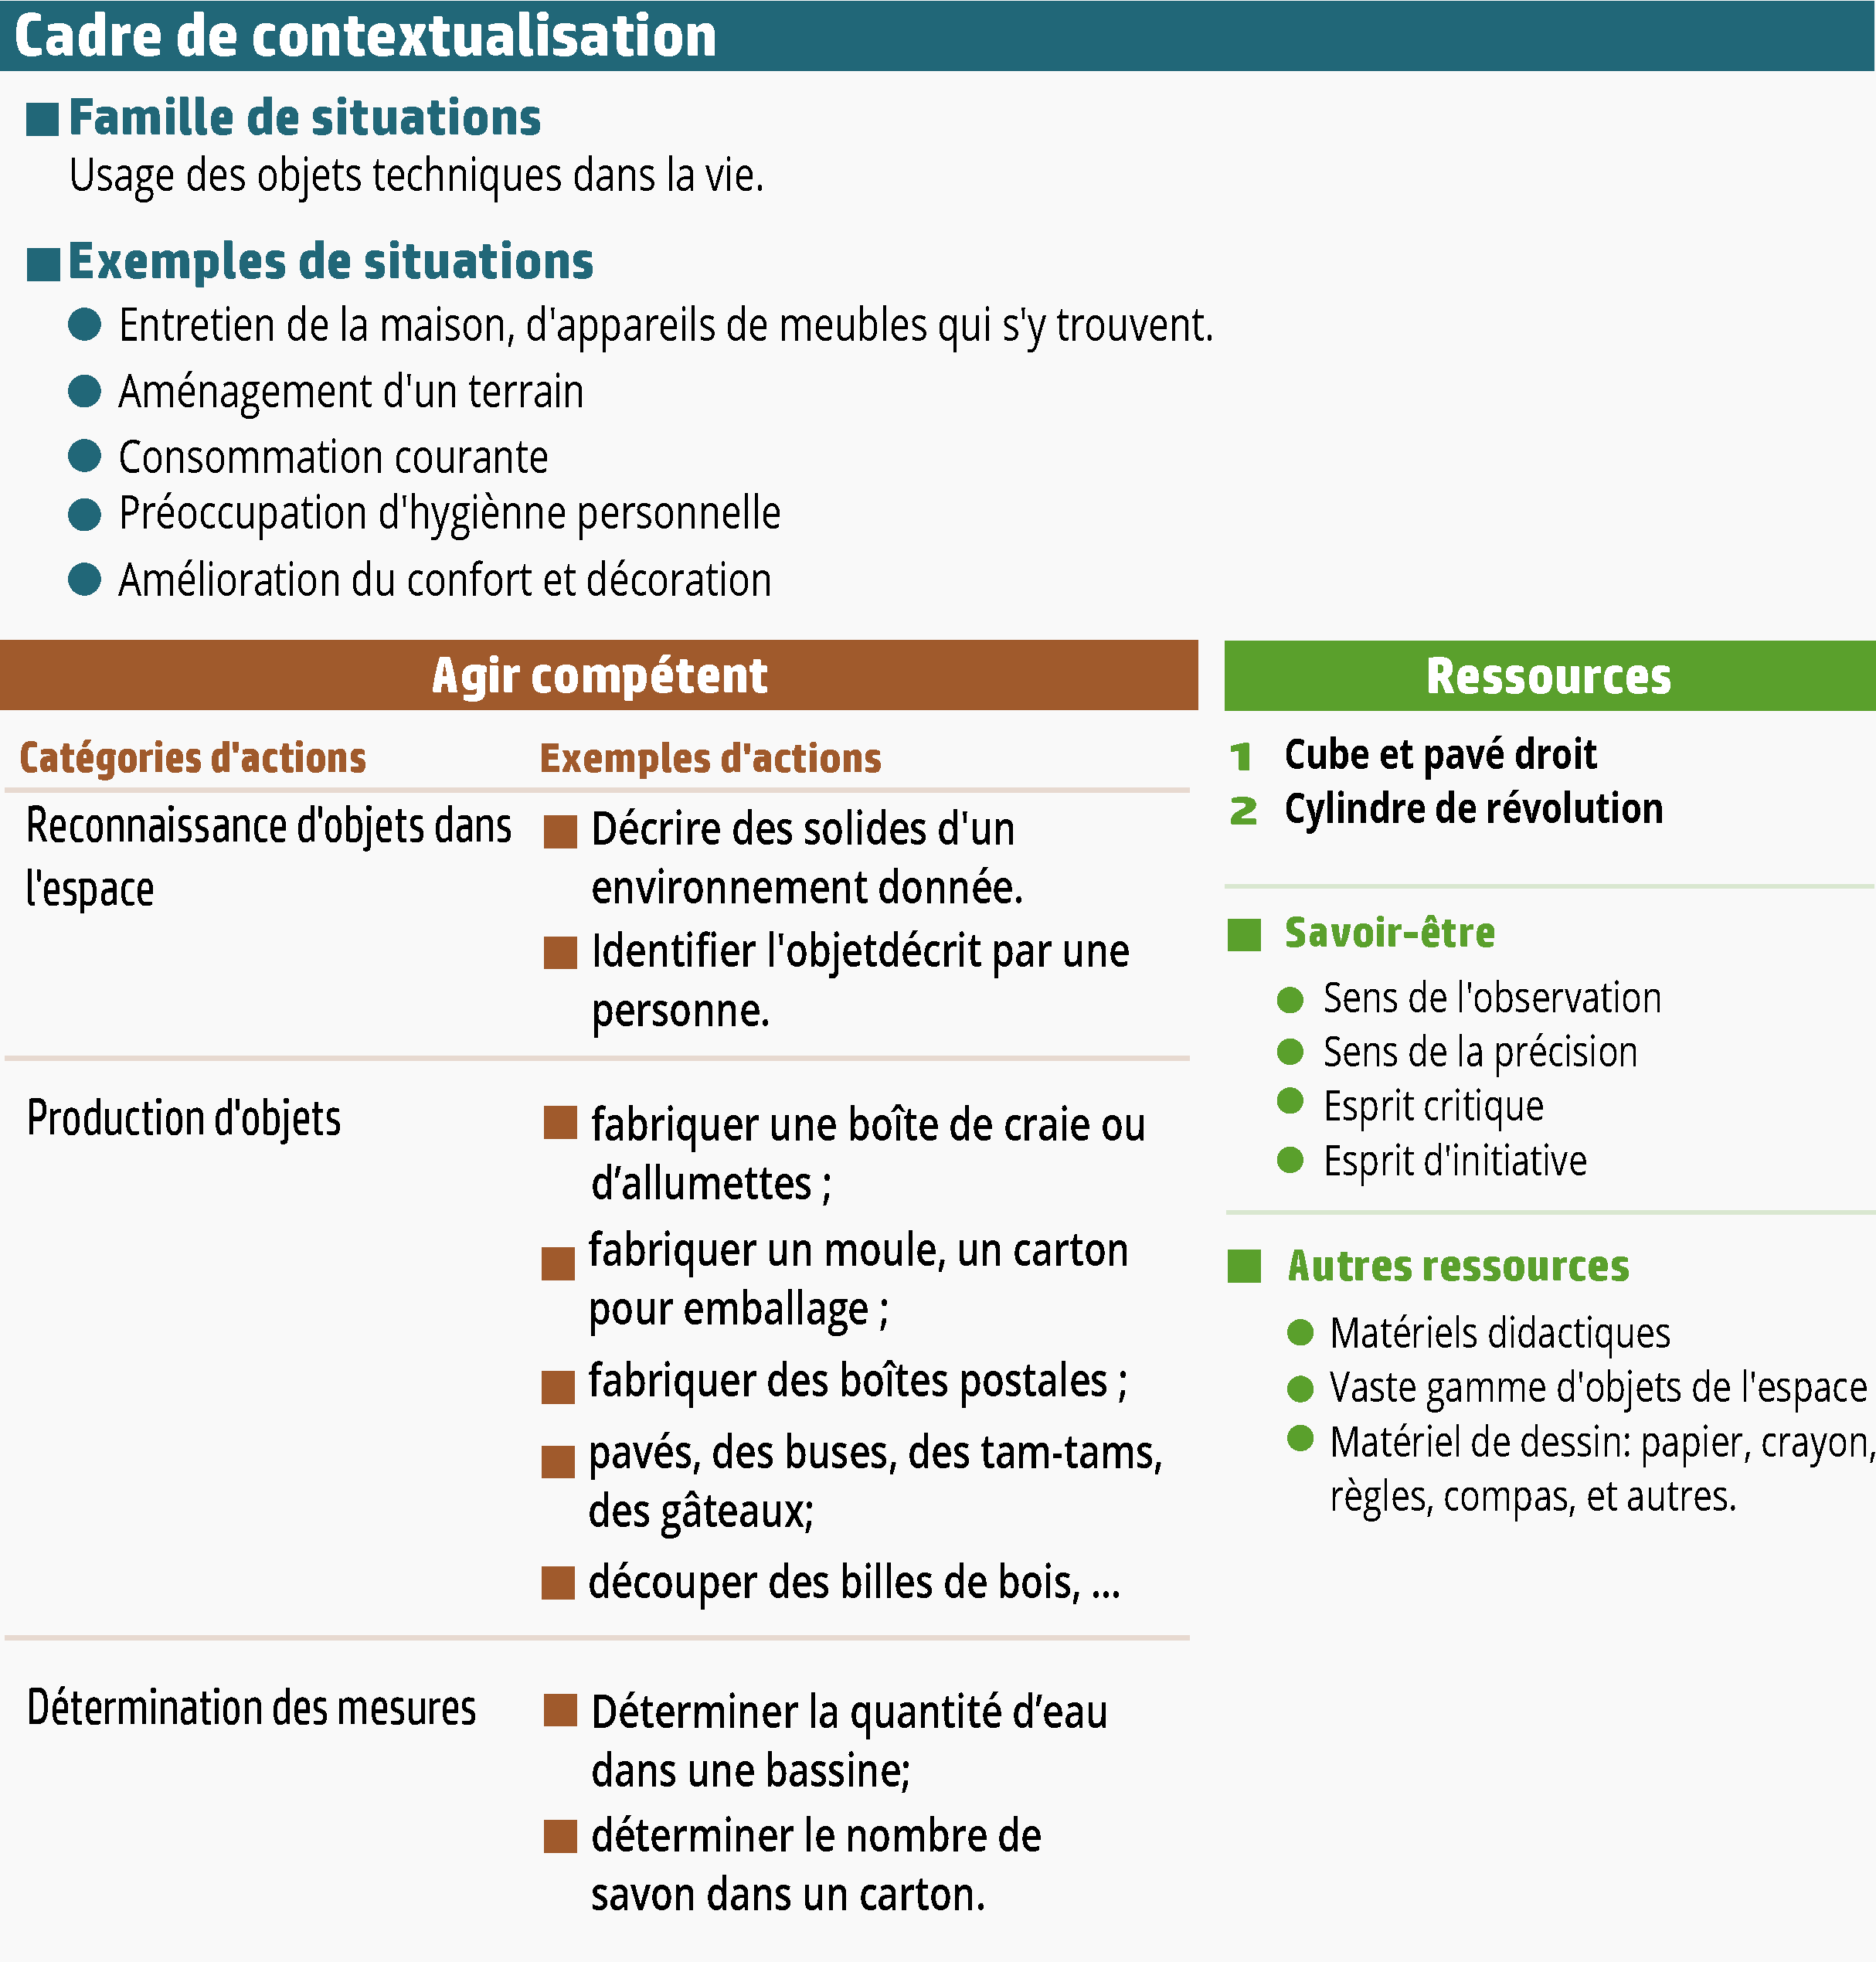
\includegraphics[width=\textwidth]{Module4.pdf} 

\subsection*{}
\addcontentsline{toc}{subsection}{\textbf{Ressource 1}: cube et pavé droit}
\ressource{Cub.pdf}

\savoir
\begin{itemize}
\item \textit{Cube et pavé droit} : forme, faces, arêtes, sommets ;
\item Propriétés:
\begin{itemize}
\item nombre de faces, d'arêtes, de sommets,
\item parallélisme de faces opposées, 
\item égalité des aires des faces opposées,
\item parallélisme des supports des arêtes opposées,
\item égalité des longueurs des arêtes opposées, 
\item perpendicularité des arêtes sécantes.
\end{itemize}
\item Volume, aire.
\end{itemize}
\savoirfaire
\begin{itemize}
\item Fabrication d'un cube, d'un pavé ; réalisation d'un patron de cube, de pavé;
\item Calcul des éléments métriques (l'aire de la surface latérale, l'aire
totale, volume) ;
\item Conversion des unités de volume.
\end{itemize}

\subsection*{}
\addcontentsline{toc}{subsection}{\textbf{Ressource 2}: cylindre de révolution}
\ressource{Cyl.pdf}

\savoir
\begin{itemize}
\item Cylindre de révolution : forme, base, surface latérale, surface de base, axe, rayon, hauteur.
\end{itemize}
\savoirfaire
\begin{itemize}
\item Fabrication d'un cylindre de révolution ;
\item Réalisation du patron ;
\item Calcul d'éléments métriques (l'aire de la surface latérale, l'aire totale et volume, hauteur, rayon de base).
\end{itemize}

\part*{Classe de cinquième}
\addcontentsline{toc}{part}{Classe de cinquième}

\chapter{Relations et opérations fondamentales dans l'ensemble des nombres décimaux et des fractions.}

{\AlegreyaSansLight \large
\begin{center}
\textbf{Crédit :} 32 heures\\
\textit{4 heures hebdomadaires}
\end{center}
}

\minitoc

\section{Introduction}
\subsection{Présentation du module}
Ce module vise à rendre l'apprenant capable de traiter de façon réussie, des situations de vie de la famille "représentation, détermination des quantités et identification des objets par des nombres ". Il s'agit en gros, de le rendre capable de :
\begin{itemize}
\item Résoudre des problèmes relatifs à des situations de vie telles que : l'achat ou la vente des biens de consommation, le partage des biens, la vérification d'une facture après payement la comparaison des prix des objets …
\item Communiquer des informations comportant des nombres (numéros de téléphones, matricule, immatriculation d'un véhicule …);
\end{itemize}
Il importe pour cela de consolider les notions d'addition, de soustraction, de multiplication de division et de relation d'ordre vues en 6ème. Les savoirs essentiels associés au présent module constituent cependant une avancée vers une habileté cognitive supérieure en l'occurrence l'application (division euclidienne, décomposition
d'un entier en produit de facteurs premiers, résolution des équations, etc.). L'enseignant pourra donc mettre un accent sur cette habileté dans les compétences liées à la résolution des problèmes.

\subsection{Contribution du module à la finalité et aux buts curriculaires}
Ce module permet de développer les compétences transversales suivantes : l'esprit critique, le sens de l'ordre et de la méthode, le sens de la rigueur et de la concision, le sens de la prévision et de l'estimation. Il contribue au renforcement de la pratique du calcul mental, à l'utilisation de la calculatrice ; ce qui permet à l'apprenant d'agir de manière autonome, compétente et adaptative dans diverses situations de la vie courante, dans lesquelles ces pratiques interviennent.

\subsection{Contribution du module au programme d'études et aux domaines de vie}
Ce module qui fait partie des programmes de mathématiques permet à chaque apprenant d'acquérir des connaissances et savoir-faire de base sur lesquels les enseignements/apprentissages qu'il recevra dans les autres disciplines du domaine d'apprentissage devront s'appuyer.\\
Les nombres décimaux sont utilisés dans toutes les sciences pour mesurer, peser et évaluer les quantités.\\
La maîtrise des concepts d'égalité, d'inégalité et des opérations fondamentales que sont l'addition, la soustraction, la multiplication et la division, est de nature à doter l'apprenant d'un certain nombre d' outils fondamentaux dont il aura besoin dans la vie pratique.\\
La gestion du budget familial, la comptabilité au sein de l'entreprise, l'évaluation des distances, des poids, des volumes, sont autant d'applications des nombres décimaux dans les domaines de vie que sont l'économie, les média, l'environnement, la santé et le bien être.

\section{Matrice}

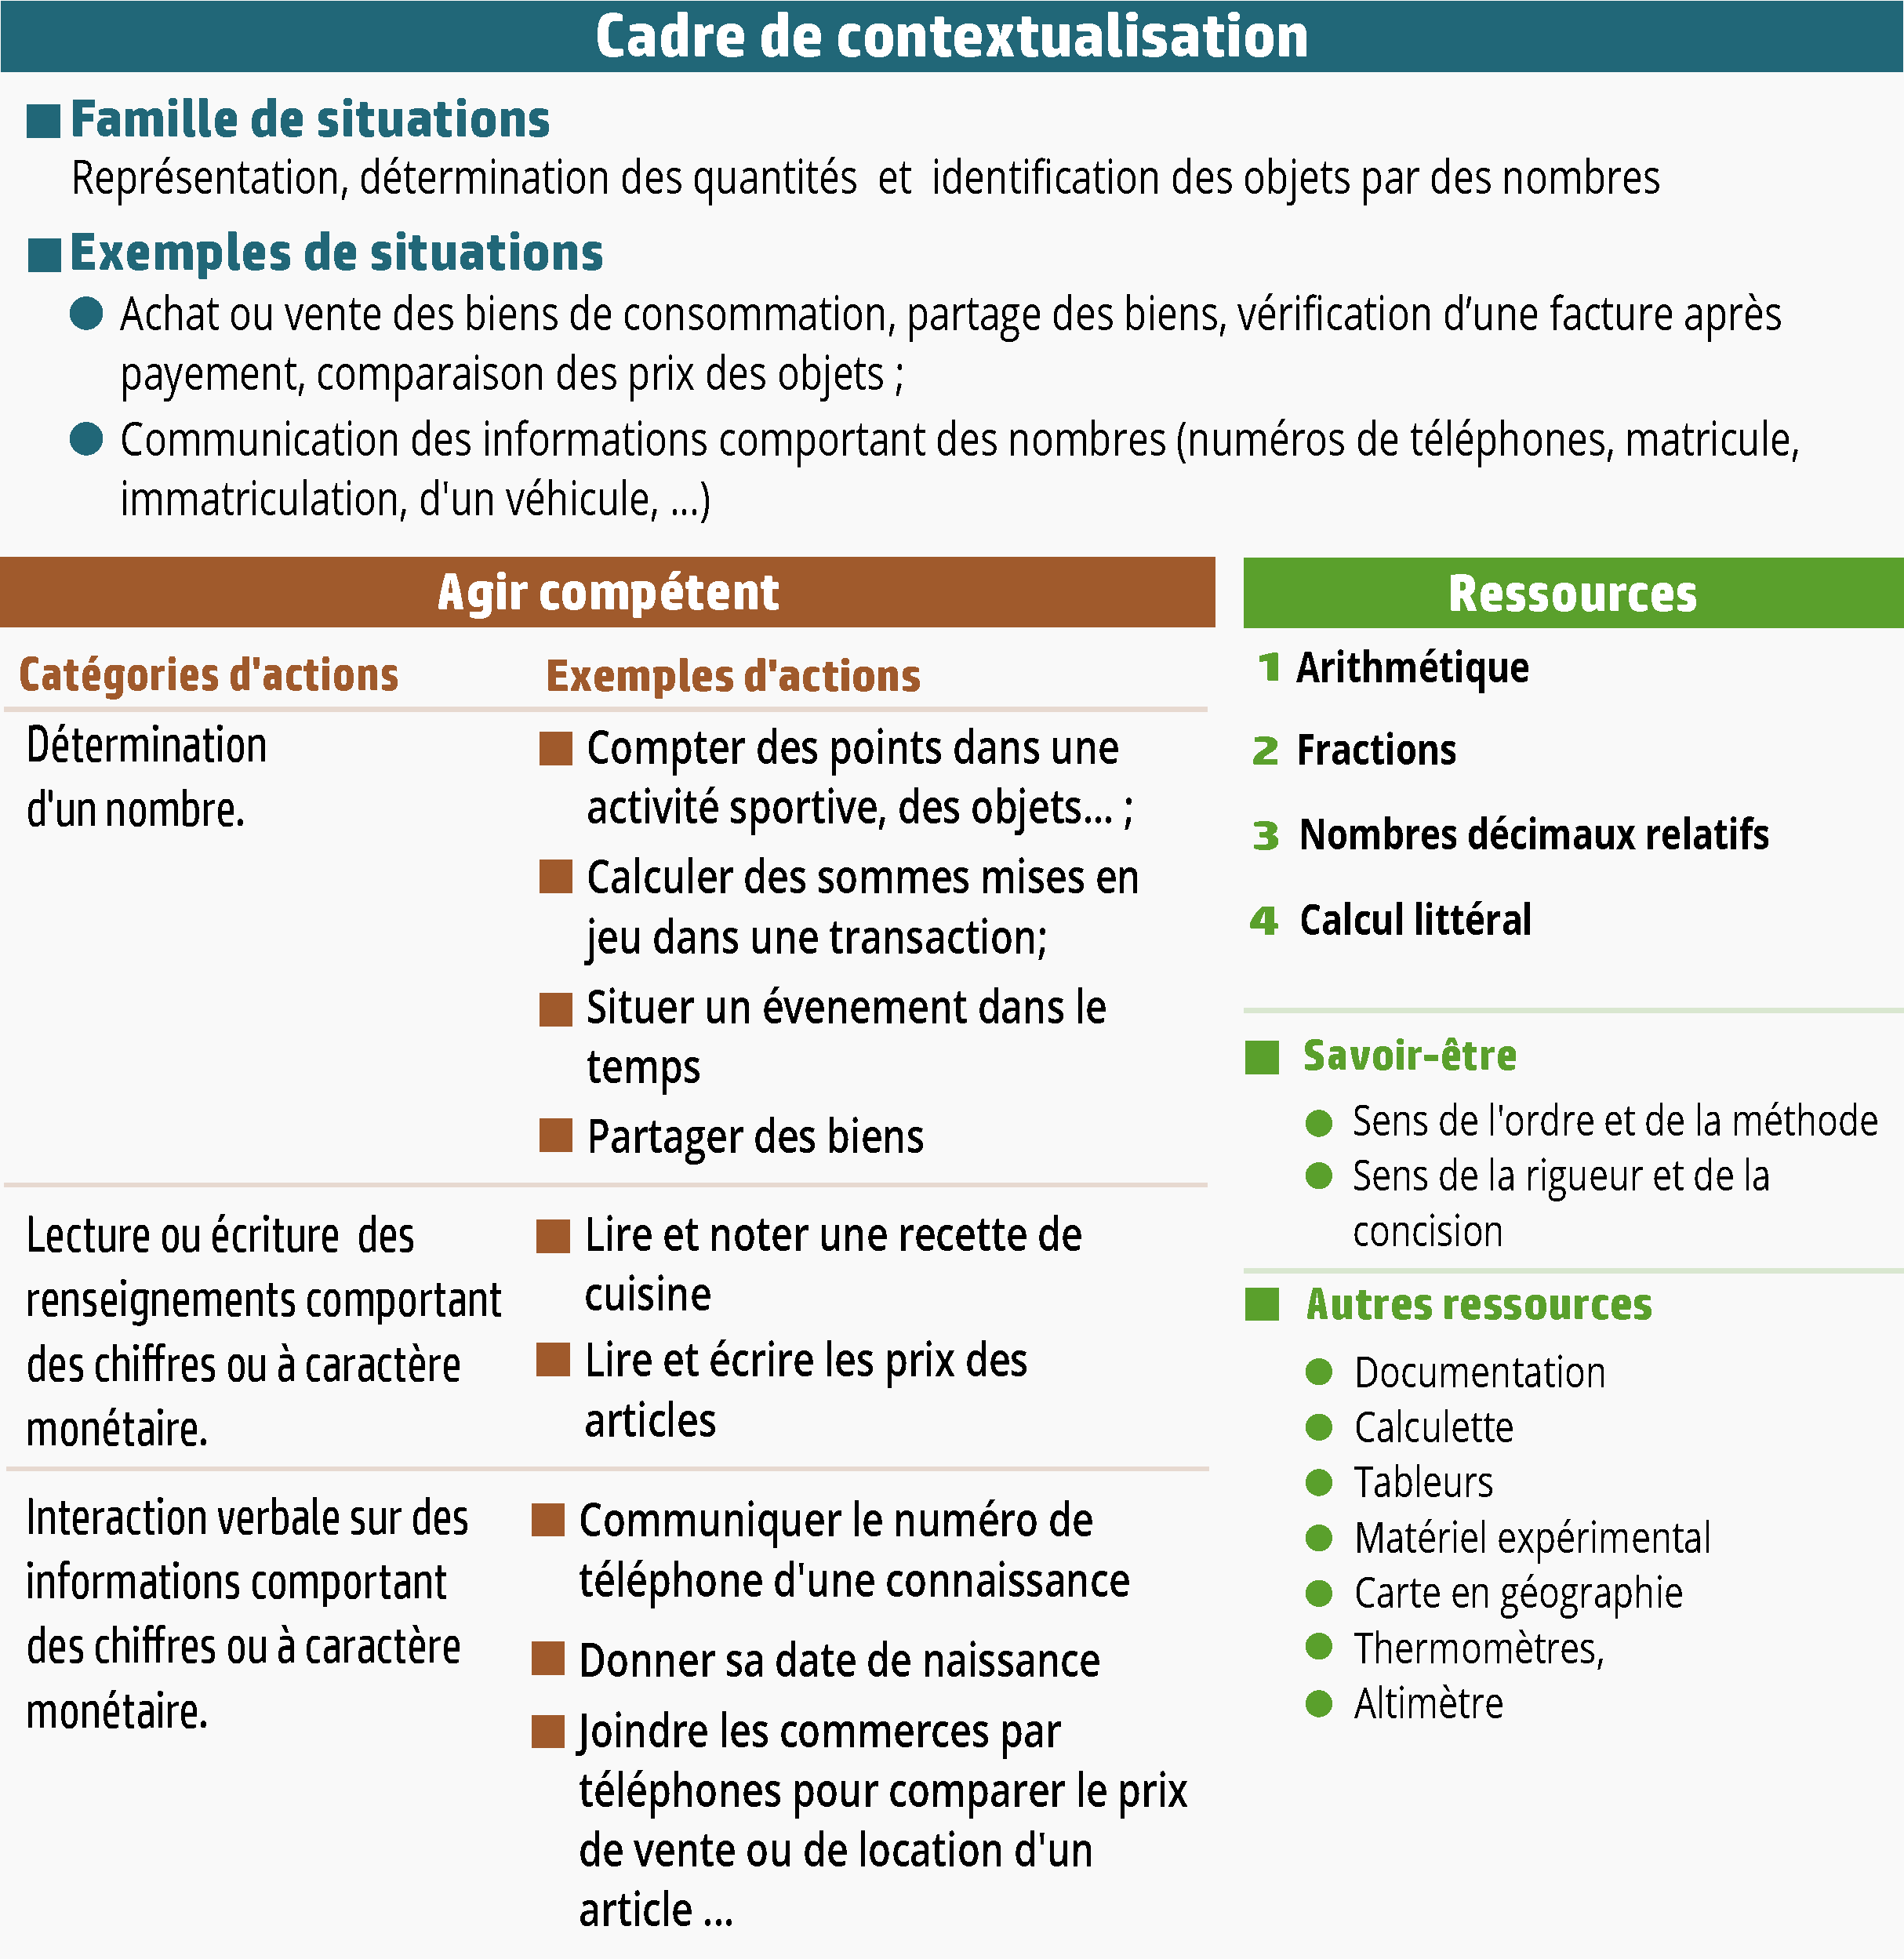
\includegraphics[width=\textwidth]{Module5.pdf} 

\subsection*{}
\addcontentsline{toc}{subsection}{\textbf{Ressource 1}: arithmétique}
\ressource{Ari.pdf}

\savoir
\begin{itemize}
\item Division euclidienne ;
\item Puissance entière d'un entier naturel ;
\item Nombres premiers ;
\item PPMC et PGDC.
\end{itemize}
\savoirfaire
\begin{itemize}
\item Décomposition en produit de facteurs premiers ;
\item Application à la recherche des multiples ou des diviseurs ;
\item Calcul du PPMC et PGDC ;
\item Critère de divisibilité : par 4 et 25.
\end{itemize}

\subsection*{}
\addcontentsline{toc}{subsection}{\textbf{Ressource 2}: fractions}
\ressource{Fractions.pdf}

\savoir
\begin{itemize}
\item Fractions irréductibles
\end{itemize}
\savoirfaire
\begin{itemize}
\item Comparaison des fractions.
\item Encadrement des fractions par deux nombres décimaux de même ordre (consécutifs) ;
\item Somme, différence, produit, division de fractions.
\end{itemize}

\subsection*{}
\addcontentsline{toc}{subsection}{\textbf{Ressource 3}: nombres décimaux relatifs}
\ressource{D5.pdf}

\savoir
\begin{itemize}
\item Opposé d'un nombre décimal relatif.
\item Puissance d'un nombre décimal relatif à exposant entier naturel non nul.
\end{itemize}
\savoirfaire
\begin{itemize}
\item Addition, soustraction, multiplication et division des nombres décimaux;
\item Calculs sur les puissances ;
\item Comparaison des nombres décimaux relatifs.
\end{itemize}

\subsection*{}
\addcontentsline{toc}{subsection}{\textbf{Ressource 4}: calcul littéral}
\ressource{CL5.pdf}

\savoir

\textbf{Equations du type:}
\begin{itemize}
\item  $a+x=b$ dans $\G D$;
\item $ax=b$ où $a$ et $b$ sont des entiers, $a$ non nul.
\end{itemize}
\chapter{Statistiques}
%\stepcounter{module}

{\AlegreyaSansLight \large
\begin{center}
\textbf{Crédit :} 11 heures\\
\textit{4 heures hebdomadaires}
\end{center}
}

\minitoc

\section{Introduction}

\subsection{Présentation du module}
Ce module vise à rendre l'apprenant capable de traiter de façon réussie, des situations de vie de la famille  "organisation des données et estimation des quantités dans la consommation des biens et services ". Il s'agit pour lui de :
\begin{itemize}
\item Déployer un raisonnement mathématique pour identifier et formaliser des situations de vie qui se rapportent aux proportionnalités.
\item Résoudre des problèmes relatifs à des situations telles que le placement d'argent, la remise au cours d'achat divers, le partage proportionnel, la collecte et l'exploitation des données, les interprétations des résultats des enquête ....
\end{itemize}
Pour y parvenir, il est nécessaire de consolider et de renforcer les acquis sur les proportionnalités, les pourcentages et l'échelle vue en sixième tout en restant sur les habiletés cognitives que sont la connaissance, la compréhension et l'application.\\
Ce module est par excellence celui qui, à ce niveau d'étude, comporte les situations de vie les plus familières à l'élève.

\subsection{Contribution du module à la finalité et aux buts curriculaires}
Le module permet de développer les compétences transversales suivantes : le sens de la concision, l'esprit critique et l'organisation rationnelle des données. A terme, ces attitudes permettent à l'apprenant de s'assumer comme membre responsable d'une famille, en même temps qu'elles lui permettent d'opérer des choix
judicieux et autonomes, dans la production, la consommation des biens et services.

\subsection{Contribution du module au programme d'études et aux domaines de vie}
Ce module est un des maillons essentiels du programme de 5ème. Il est par excellence lui-aussi, le domaine d'intégration des mathématiques dans la vie quotidienne. Les situations de vie et les exemples de situations auxquelles il renvoie, de même que toutes les autres composantes du module pourront tout aussi bien
intervenir en physique, dans les sciences de la vie et de la terre, en géographie, et plus tard en psychologie et en économie, pour ne citer que ces disciplines-là. Il permet à ce niveau de dégager de manière implicite et même transversale l'importance de l'interdisciplinarité dans plus d'un domaine d'apprentissage.\\
La maîtrise de cette notion que ce module développe est de nature à doter l'apprenant d'outils essentiels dont il a besoin dans la vie pratique. Sa contribution dans la gestion du budget familiale est indéniable. Son implication dans la détermination des quantités justifie son importance dans la consommation des biens. Une bonne maîtrise des statistiques situées est un atout majeur dans la consommation des informations, et dans l'exploitation, l'analyse et l'interprétation des données à caractère économique ou social.

\section{Matrice}

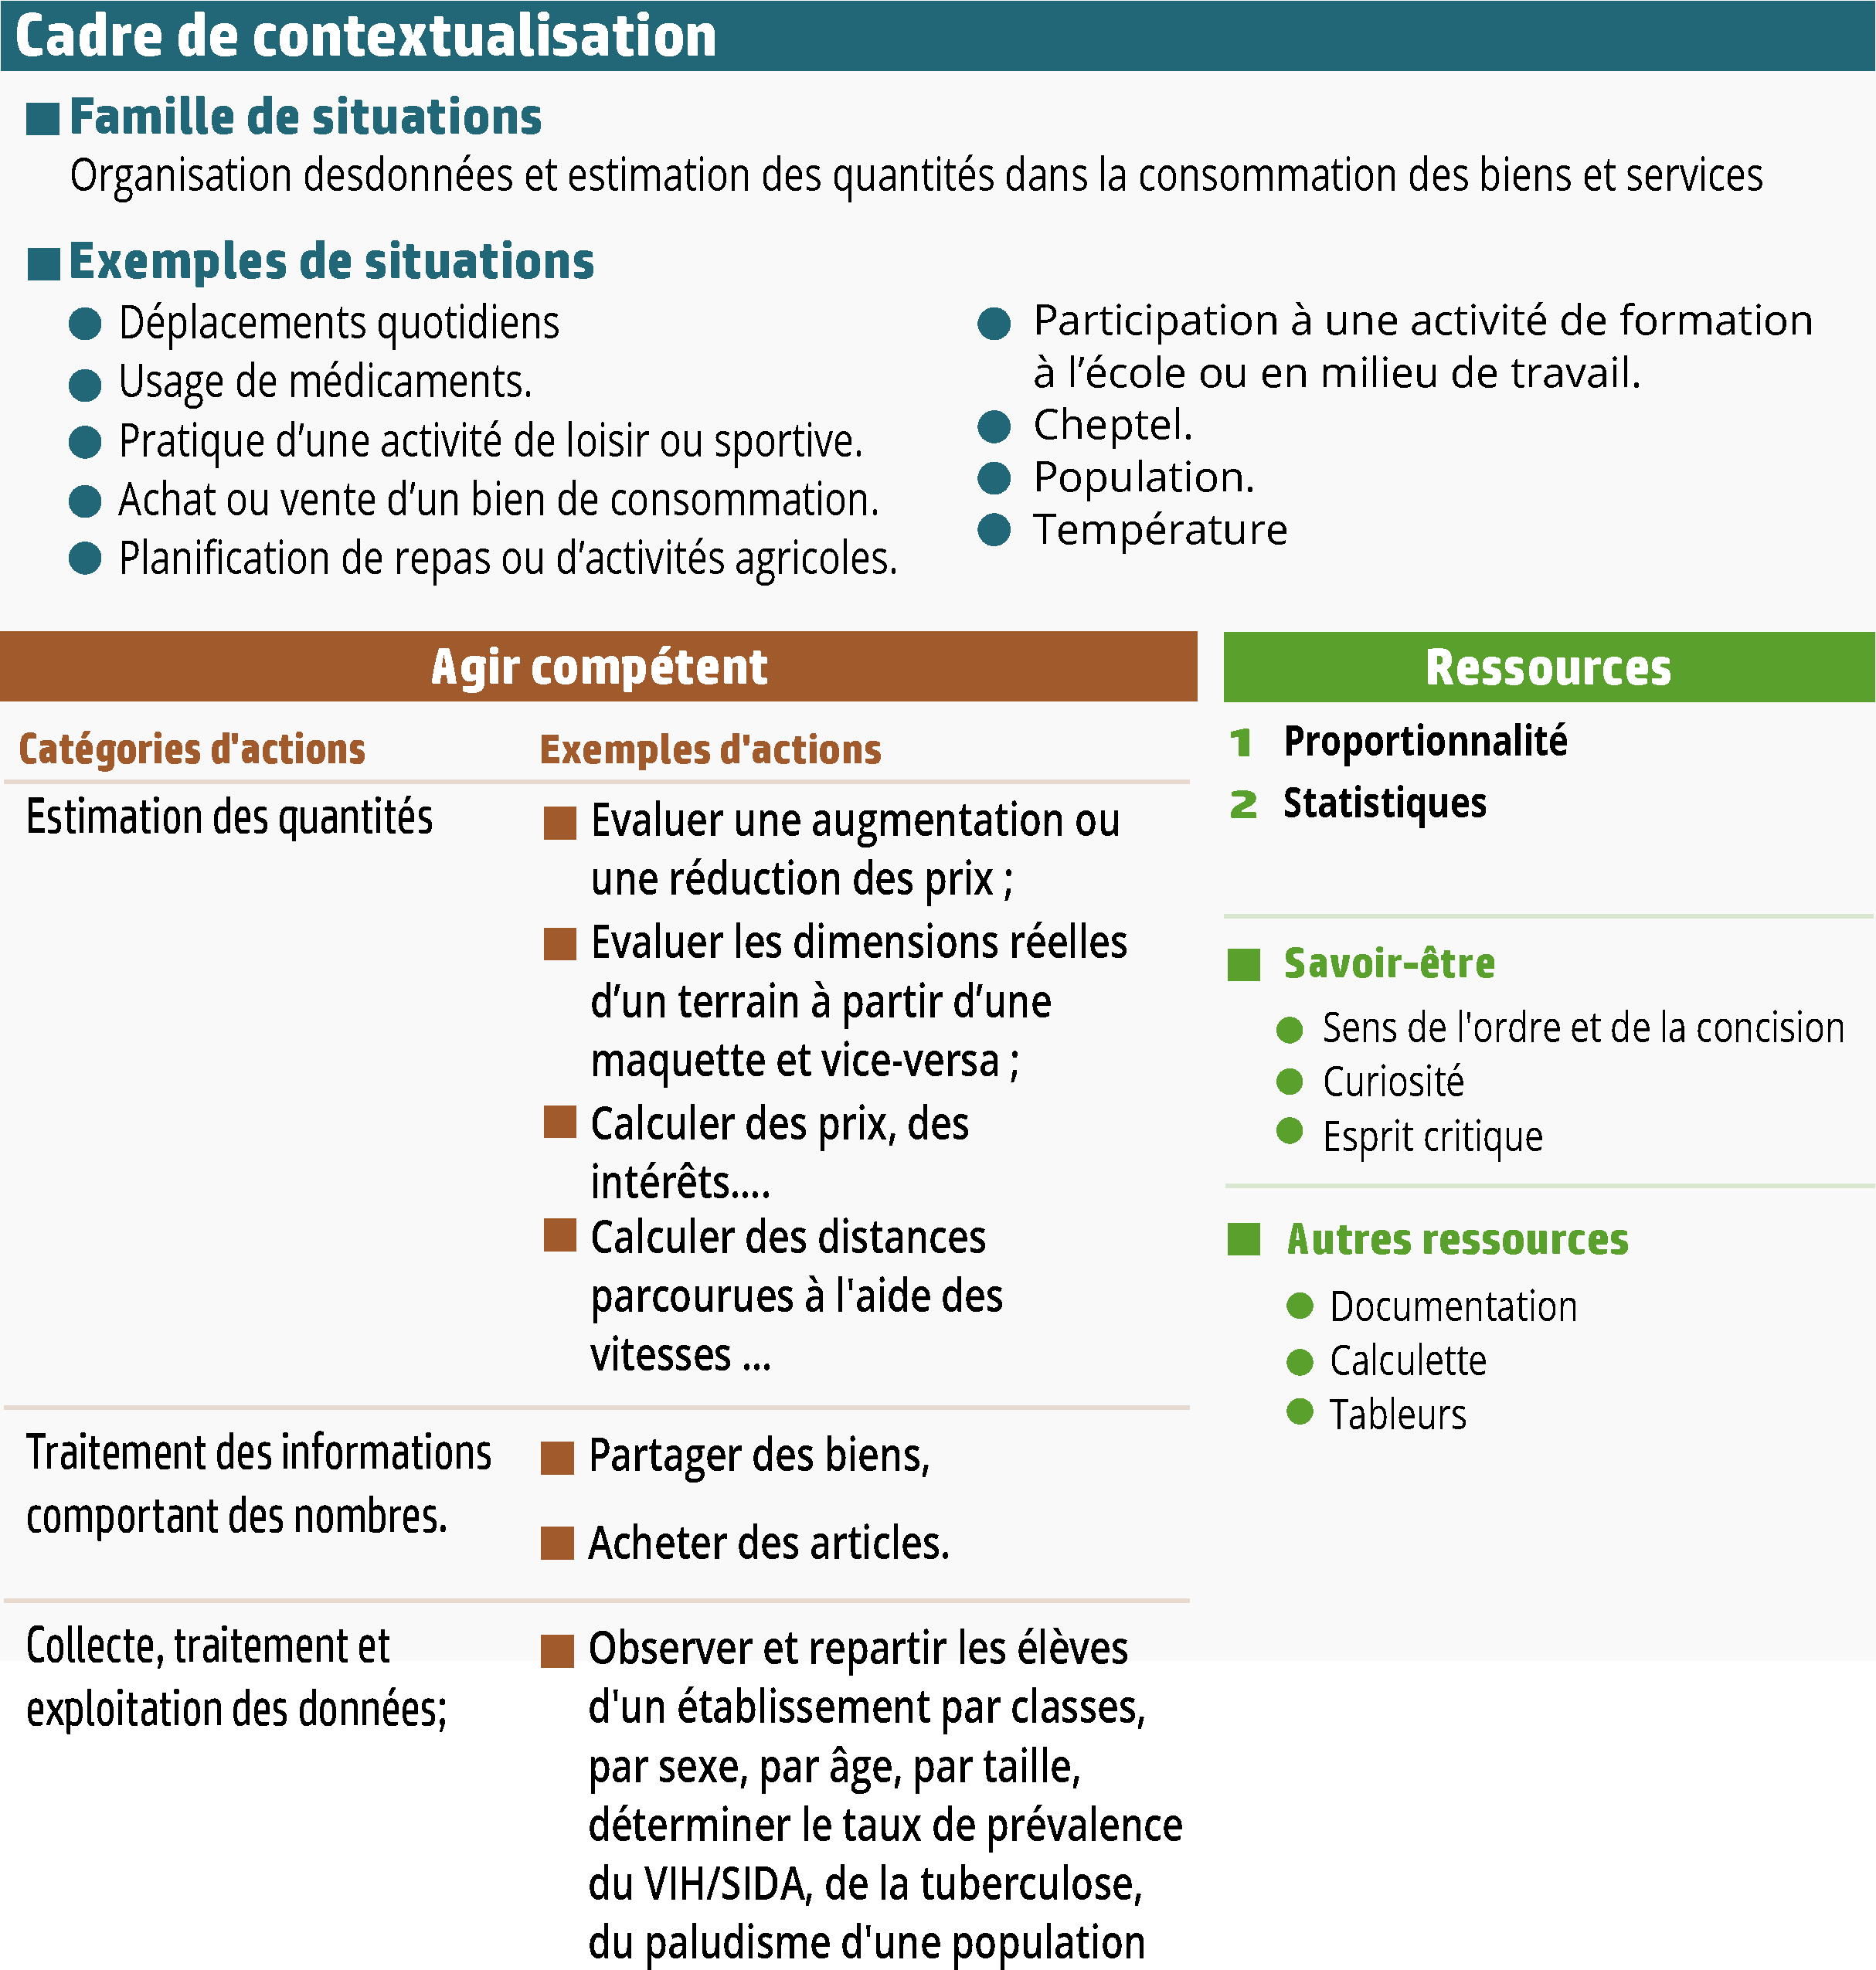
\includegraphics[width=\textwidth]{Module6.pdf} 

\subsection*{}
\addcontentsline{toc}{subsection}{\textbf{Ressource 1}: proportionnalité}
\ressource{Prop.pdf}

\savoir
\begin{itemize}
\item Coefficient de proportionnalité
\end{itemize}
\savoirfaire
\begin{itemize}
\item Calcul d'un coefficient de proportionnalité particulier : vitesse, masse volumique, débit.
\item Calcul d'un pourcentage, d'une échelle.
\item Représentation graphique d'une situation de proportionnalité dans un quadrillage.
\item Identification et exploitation du graphique d'une situation de proportionnalité dans un quadrillage.
\end{itemize}

\subsection*{}
\addcontentsline{toc}{subsection}{\textbf{Ressource 2}: statistiques}
\ressource{Stat.pdf}

\savoir
\begin{itemize}
\item \textit{Vocabulaire:} population, caractère, modalité, effectif d'une population, effectif d'une modalité.
\item Fréquences
\end{itemize}
\savoirfaire
\begin{itemize}
\item Elaboration d'un tableau des effectifs et des fréquences en pourcentage.
\end{itemize}
\chapter{Configurations et transformations élémentaires du plan}
%\stepcounter{module}

{\AlegreyaSansLight \large
\begin{center}
\textbf{Crédit :} 46 heures\\
\textit{4 heures hebdomadaires}
\end{center}
}

\minitoc

\section{Introduction}

\subsection{Présentation du module}
Ce module comporte deux parties essentielles : les configurations planes, les symétries orthogonales et centrales dans le plan. Il développe deux compétences fondamentales que sont :
\begin{itemize}
\item déployer un raisonnement mathématique (analogique, inductif et déductif);
\item résoudre des problèmes par l'observation, l'identification et la caractérisation des formes planes ; par les transformations élémentaires que sont les symétries.
\end{itemize}
Il s'articule sur la famille de situations suivante : représentations et transformations des configurations planes dans l'environnement. Les compétences mises en contexte s'appuient sur les trois catégories d'actions que sont :
\begin{itemize}
\item Perception des formes planes et des transformations dans l'environnement physique.
\item Production des formes planes et des transformations dans l'environnement physique.
\item Détermination des mesures et des positions dans l'environnement.\\
Cette dernière catégorie d'actions est le champ privilégié de l'inter action entre les activités numériques et les activités géométriques de l’élève de 5ème .\\
Les différentes actions qui s'intègrent dans chacune des catégories suscitées sont en corrélation avec les savoirs essentiels que ce module développe, et qui s'appuient sur les habiletés cognitives suivantes : connaissance, compréhension et application.
\end{itemize}

\subsection{Contribution du module à la finalité et aux buts curriculaires}
A travers les différents raisonnements sus évoqués, l'apprenant développe les compétences transversales suivantes : le sens de l'ordre, le sens de la rigueur et de la concision (en intégrant, dans le cadre d'une démarche scientifique, chacune des méthodes utilisées pour le traitement compétent des situations de vie), la pensée
critique, le sens de l'initiative et de la créativité. Autant d'attitudes qui contribuent à la formation d'un citoyen autonome et responsable dans l'exercice de ses rôles sociaux.

\subsection{Contribution du module au programme d'études et aux domaines de vie}
La géométrie plane occupe une place privilégiée dans le programme de mathématiques de par les compétences qu'elle vise à développer. Sa contribution au développement de la technologie, de l'art, de la chimie, ne sont plus à démontrer ; enfin les innombrables symétries que la nature offre dans la biologie et la physiologie végétale ou animale font de ce module un des maillons essentiels dans plus d'un domaine d'apprentissage.\\
L'importance de ce module réside dans le fait que l'élève vit dans un espace géographique. L'utilisation et la rencontre des objets dans lesquels on peut extraire des formes géométriques planes font partie du quotidien : aménagement ou réalisation de son habitat, manipulation ou réalisation de certains objets usuels, appréciation ou production des œuvres d'art, choix du chemin adéquat pour se rendre à un lieu pour ne citer que ceux-ci ; toutes choses pouvant l'aider à s'affirmer comme membre responsable d'une famille, à opérer des choix judicieux dans la consommation des biens , des services et de l'information. La contribution de ce module à tous les domaines de vie est donc d'une évidence incontestable.

\section{Matrice}

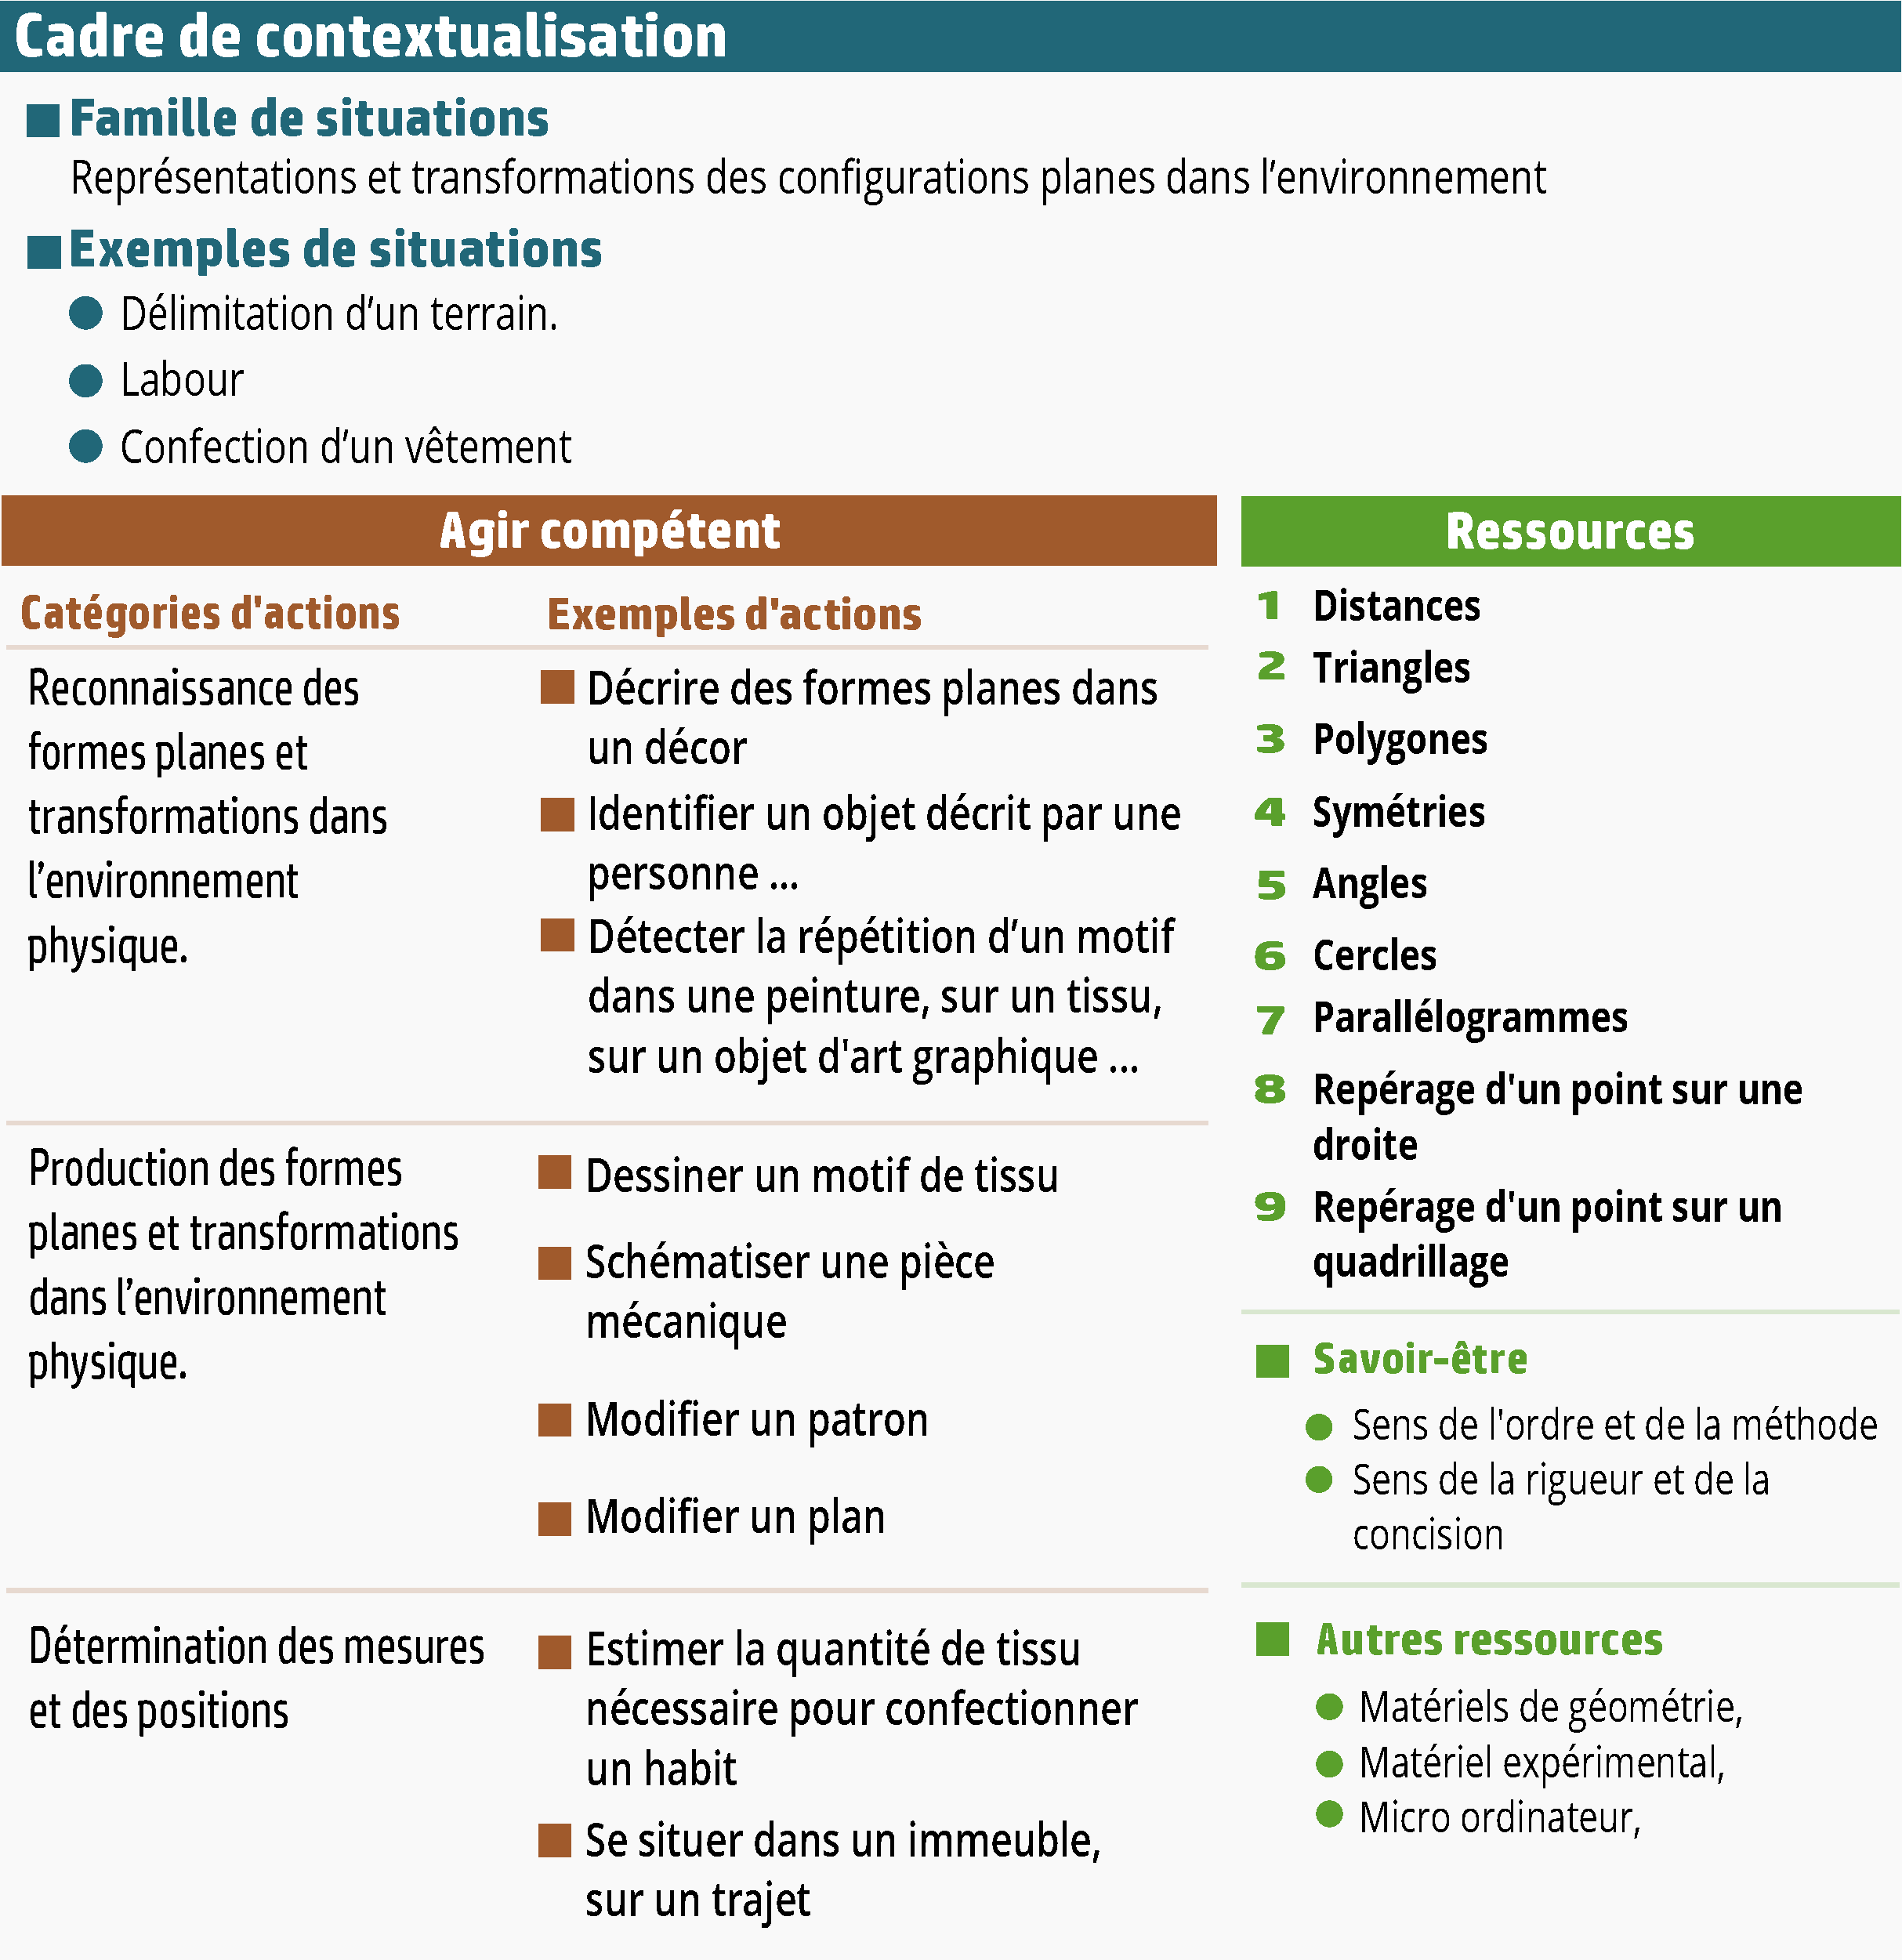
\includegraphics[width=\textwidth]{Module7.pdf} 

\subsection*{}
\addcontentsline{toc}{subsection}{\textbf{Ressource 1}: distances}
\ressource{Dis.pdf}

\savoir
\begin{itemize}
\item Distances de deux points.
\item Inégalité triangulaire.
\item  Caractérisation d'un segment par les distances (Si $M\in\ife{AB}$ alors  MA + MB = AB et si $MA+MB=AB$
alors $M\in\ife{AB}$ ).
\item Caractérisation de la médiatrice d'un segment par l'égalité des distances.
\end{itemize}
\savoirfaire
\begin{itemize}
\item Construire la médiatrice d'un segment à la règle et au compas.
\item Utiliser l'inégalité triangulaire et la caractérisation de la médiatrice pour justifier des inégalités ou des égalités des distances.
\end{itemize}

\subsection*{}
\addcontentsline{toc}{subsection}{\textbf{Ressource 2}: triangles}
\ressource{Tri5.pdf}

\savoir
\begin{itemize}
\item \textit{ Droites particulières dans un triangle} : hauteur, médiatrice, médiane, bissectrice.
\item Somme des angles d'un triangle.
\item \textit{Caractérisation des triangles particuliers}: triangle rectangle, triangle isocèle, triangle équilatéral.
\end{itemize}
\savoirfaire
\begin{itemize}
\item Construction des triangles particuliers.
\item Construction des droites particulières d'un triangle (hauteurs, médiatrices, médianes, bissectrices).
\end{itemize}

\subsection*{}
\addcontentsline{toc}{subsection}{\textbf{Ressource 3}: polygones}
\ressource{Pol.pdf}

\savoir
\begin{itemize}
\item \textit{Polygones usuels} : triangle, trapèze, pentagone, hexagone régulier, octogone régulier, parallélogrammes.
\end{itemize}
\savoirfaire
\begin{itemize}
\item \textit{Caractérisation des polygones particuliers en liaison avec les symétries} : trapèze isocèle, hexagone
régulier, octogone régulier.
\item \textit{Reconnaître et construire un polygone particulier} : parallélogramme, trapèze, losange, hexagone régulier, octogone régulier, pentagone.
\end{itemize}

\subsection*{}
\addcontentsline{toc}{subsection}{\textbf{Ressource 4}: symétries}
\ressource{Sym.pdf}

\savoir
\begin{itemize}
\item Symétries par rapport à un point, symétrie orthogonale.
\item \textit{Propriétés de conservation} : distances, angles, formes, parallélisme, orthogonalité, alignement des points.
\end{itemize}
\savoirfaire
\begin{itemize}
\item Construction des figures symétriques par rapport à une droite ou un point (point, droite, segment, triangle, cercle) ;
\item Utilisation des propriétés de conservation pour justifier une égalité de distance ou angulaire ou l'alignement de 3 points, l'orthogonalité ou le parallélisme de 2 droites ;
\item Remplir un tableau de correspondance dans l'étude des figures symétriques ;
\item Reconnaître une configuration admettant un axe(ou un centre) de symétrie et préciser cet axe (ou ce centre) de symétrie.
\end{itemize}

\subsection*{}
\addcontentsline{toc}{subsection}{\textbf{Ressource 5}: angles}
\ressource{Ang5.pdf}

\savoir
\begin{itemize}
\item Angles complémentaires, angles supplémentaires ;
\item Angles opposés par le sommet ;
\item Angles formés par deux droites parallèles et une sécante ;
\item Angles alternes - internes, angles alternes-externes, angles correspondants.
\end{itemize}
\savoirfaire
\begin{itemize}
\item Utiliser les différentes propriétés pour justifier une égalité angulaire.
\end{itemize}

\subsection*{}
\addcontentsline{toc}{subsection}{\textbf{Ressource 6}: cercle}
\ressource{Cer5.pdf}

\savoir
\begin{itemize}
\item Cercle circonscrit à un triangle, à un rectangle ;
\item \textit{Régionnement du plan par un cercle}: intérieur, extérieur d'un cercle
\end{itemize}
\savoirfaire
\begin{itemize}
\item Position d'un point par rapport à un cercle ;
\item Construction du cercle circonscrit à un triangle, à un rectangle.
\end{itemize}

\subsection*{}
\addcontentsline{toc}{subsection}{\textbf{Ressource 7}: repérage d'un point sur une droite}
\ressource{Repd.pdf}

\savoir
\begin{itemize}
\item Notion d'abscisse relativement d'un point.
\end{itemize}
\savoirfaire
\begin{itemize}
\item Justifier des inégalités de nombre par leur rangement sur une droite.
\end{itemize}

\subsection*{}
\addcontentsline{toc}{subsection}{\textbf{Ressource 8}: repérage d'un point sur un quadrillage}
\ressource{Repq.pdf}

\savoir
\begin{itemize}
\item Vocabulaire ;
\item Notion de couple de coordonnées (entiers relatifs).
\end{itemize}
\savoirfaire
\begin{itemize}
\item Placer sur un quadrillage, un point dont on connaît le couple de coordonnées (entiers relatifs) ;
\item Lire le couple de coordonnées d'un point dans un quadrillage.
\end{itemize}  


\chapter{Solides de l'espace}
%\stepcounter{module}

{\AlegreyaSansLight \large
\begin{center}
\textbf{Crédit :} 11 heures\\
\textit{4 heures hebdomadaires}
\end{center}
}

\minitoc

\section{Introduction}

\subsection{Présentation du module}
Ce module comporte deux parties essentielles : prismes droits et sphère. Il développe deux compétences fondamentales que sont :
\begin{itemize}
\item déployer un raisonnement mathématique (analogique, inductif et déductif)
\item résoudre des problèmes par l'observation, l'identification et la caractérisation des objets de l'espace.
\end{itemize}
Il s'articule sur la famille de situations suivante : usage des objets techniques dans la vie. Les compétences mises en contexte s'appuient sur les trois catégories d'actions qui suivent :
\begin{itemize}
\item Reconnaissance des solides dans l'espace.
\item Production d'objets.
\item Détermination des mesures.
\end{itemize}
Cette dernière catégorie d'actions est le champ privilégié de l'inter action entre les activités numériques et les activités géométriques de l'élève de 5ème.\\
Les différentes actions qui s'intègrent dans chacune des catégories suscitées sont en corrélation avec les savoirs essentiels que ce module développe, et qui s'appuient sur les habiletés cognitives suivantes : connaissance, compréhension et application.
\subsection{Contribution du module à la finalité et aux buts curriculaires}
L'apprentissage de la géométrie en général, et de la géométrie dans l'espace en particulier concourt à la construction du raisonnement, à la familiarisation avec les techniques calculatoires telles que les calculs d'aires et des volumes. Le traitement de la famille de situations aidera l'élève à construire ces éléments de formation. Il pourra également se familiariser avec les techniques de classement, d'observation et de description, de représentation, autant d'attitudes qui contribuent à l'autonomie.
\subsection{Contribution du module au programme d'études et aux domaines de vie}
Les éléments de formation que l'élève construira en traitant avec compétence la famille de situations choisie devrait l'aider à réaliser des actions et résoudre des problèmes.\\
De plus, le présent module est d'un apport significatif au domaine d'apprentissage intitulé « sciences et technologie », tant il participe à la conception, à la représentation, et à la réalisation des chefs d'œuvres architecturaux, et de tous les objets technologiques qui nous entourent. Sa contribution à la représentation
de la structure cristalline de certains éléments de base en chimie mérite elle aussi d'être soulignée. Enfin il ne serait pas superflu de signaler sa contribution au développement des arts plastiques et graphiques, véhicules de grandes valeurs universelles telles que l'esthétique et l'harmonie.\\
La contribution de ce module au développement de la technologie vient d'être soulignée plus haut. L'importance du développement de la technologie n'est plus à démontrer dans la vie économique, et dans l'amélioration du bien être familial. On peut donc affirmer par voie de conséquence que la contribution de ce module à la vie sociale et familiale, et surtout à la vie économique est déterminante. Cette contribution peut même être étendue, de manière implicite au domaine de la citoyenneté, et à celui des arts.

\section{Matrice}

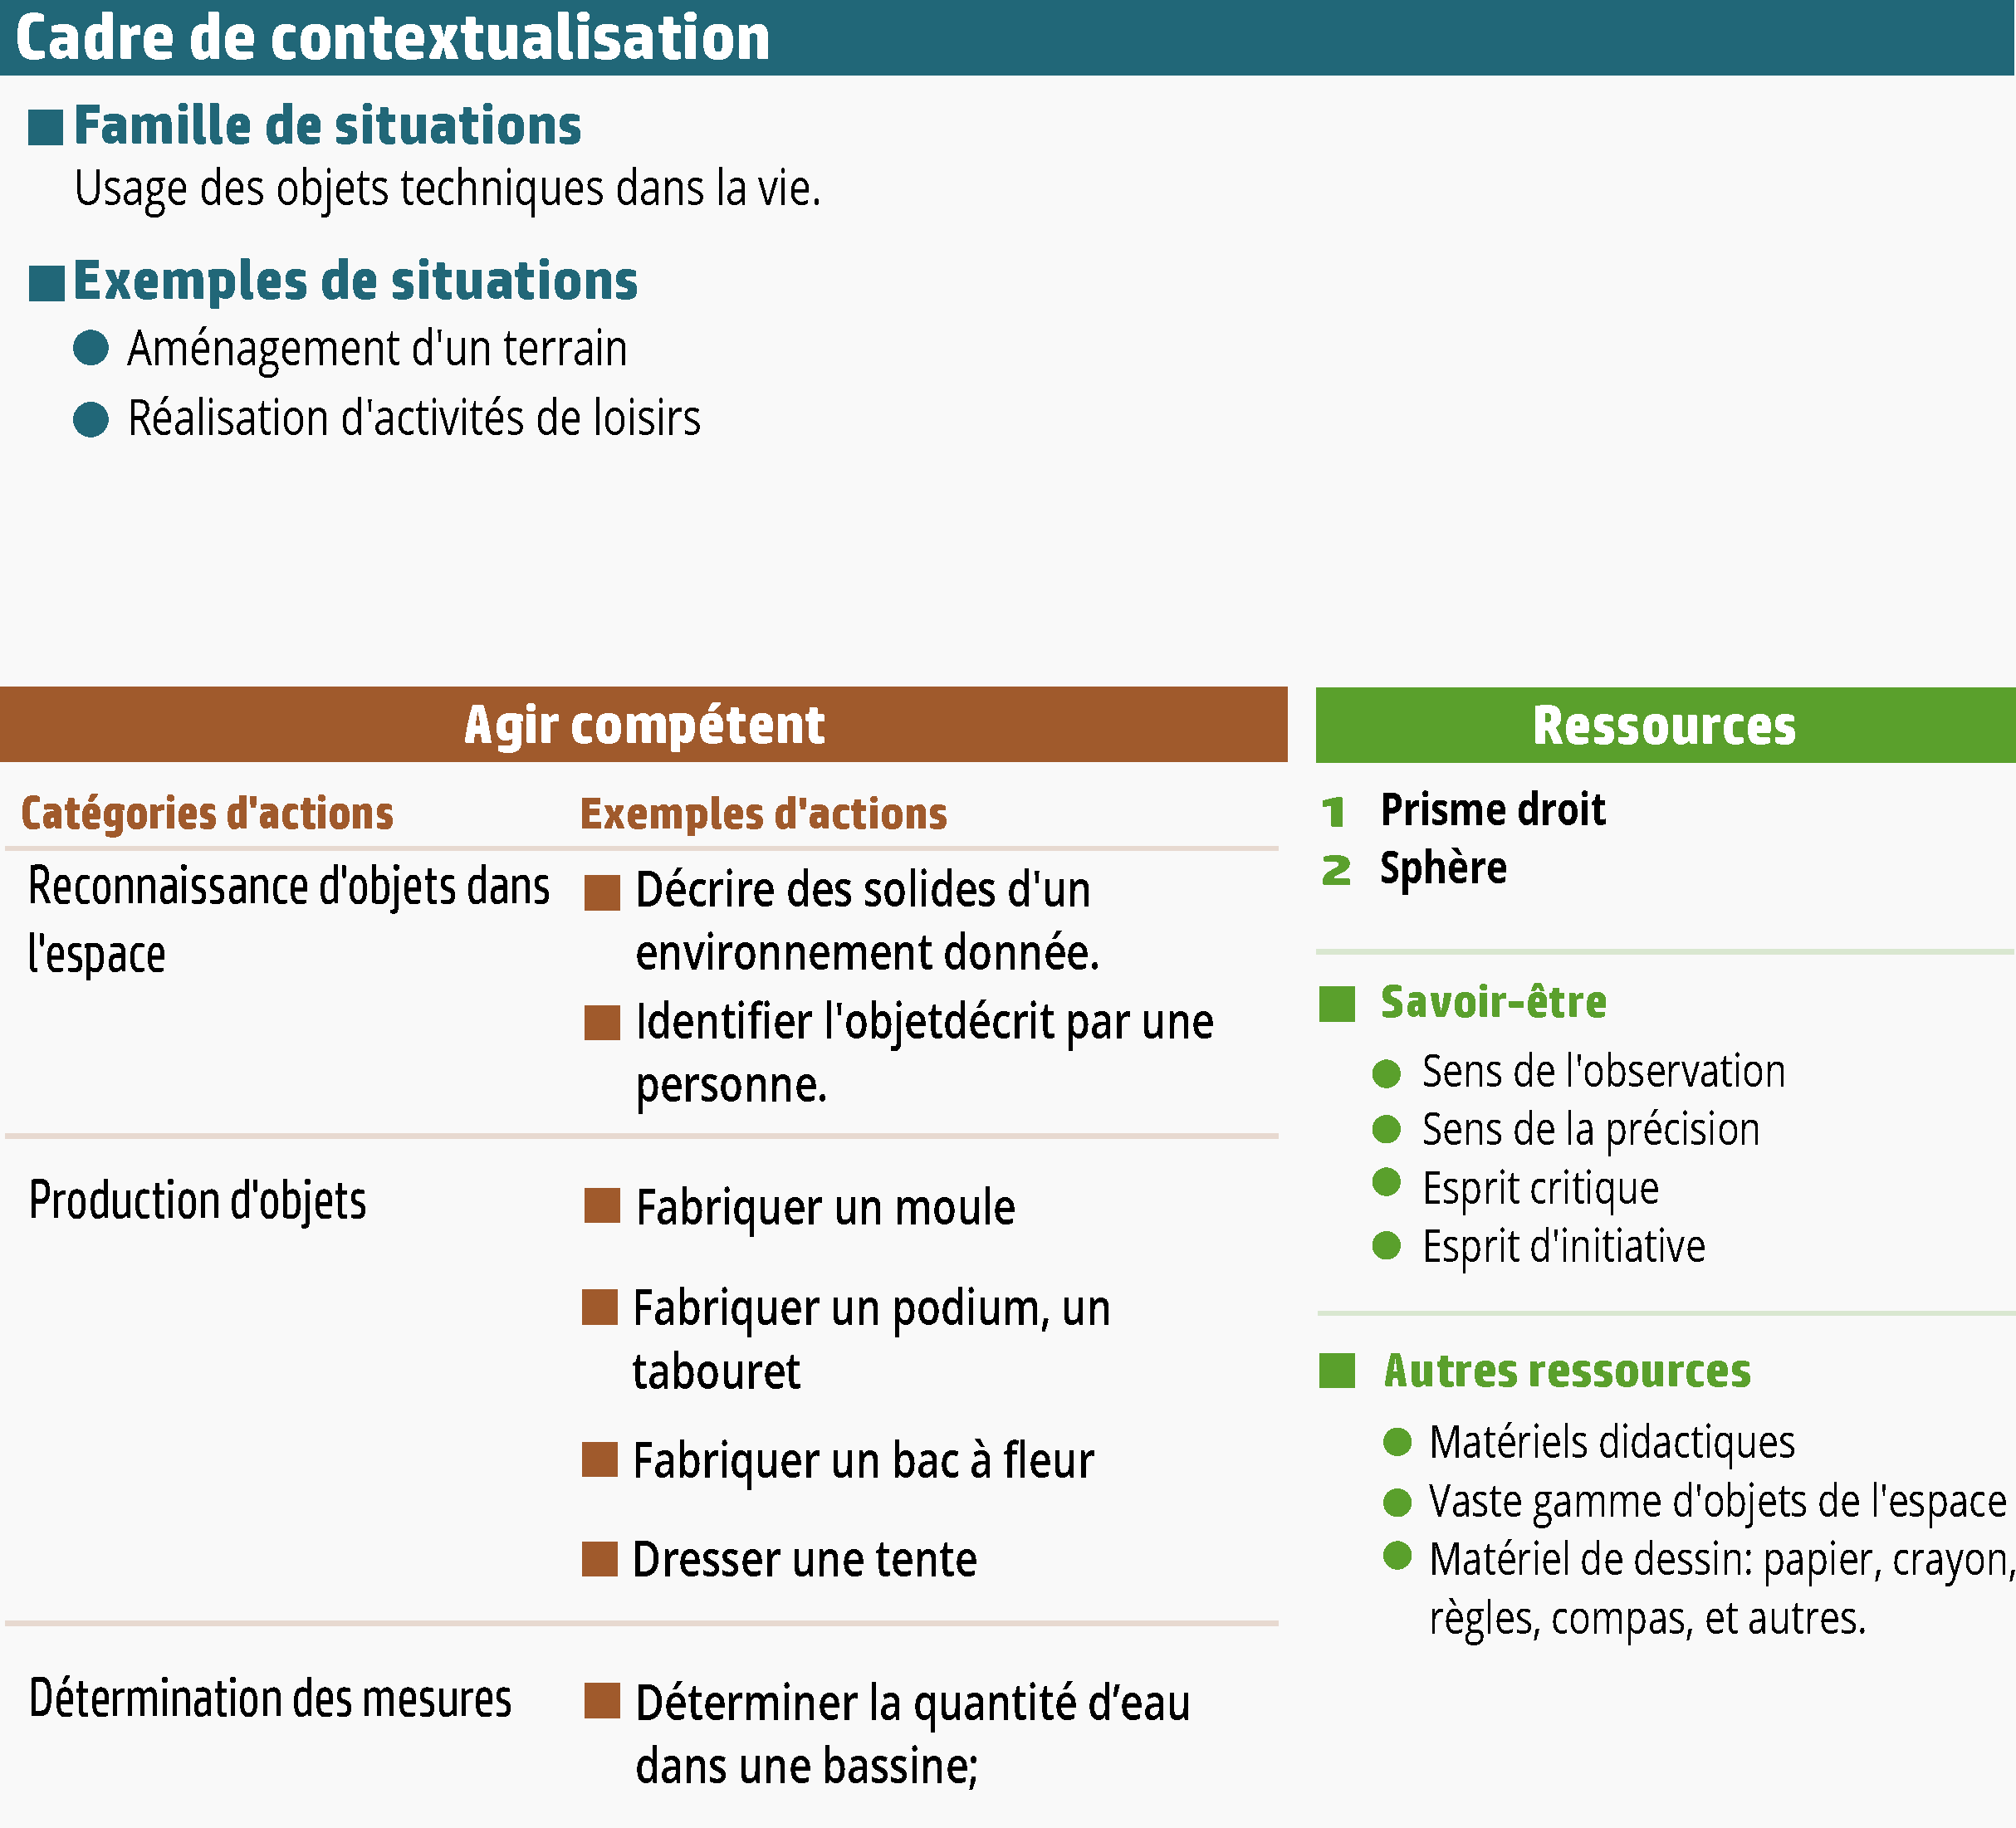
\includegraphics[width=\textwidth]{Module8.pdf} 

\subsection*{}
\addcontentsline{toc}{subsection}{\textbf{Ressource 1}: prisme droit}
\ressource{Pri.pdf}

\savoir
\begin{itemize}
\item \textit{Prisme droit} : forme, faces, bases, arêtes ;
\item \textit{Propriétés}: nombre de faces, d'arêtes, de sommets,
\item \textit{Eléments métriques}: aire latérale, aire totale, volume.
\end{itemize}
\savoirfaire
\begin{itemize}
\item Fabrication d'un prisme droit et réalisation d'un patron d'un prisme droit;
\item Calcul des éléments métriques (l'aire de la surface latérale, l'aire
totale, volume) ;
\end{itemize}

\newpage

\subsection*{}
\addcontentsline{toc}{subsection}{\textbf{Ressource 2}: sphère}
\ressource{Sph.pdf}

\savoir
\begin{itemize}
\item Sphère et boule : forme, centre, rayon, diamètre;
\item Eléments métriques : aire d"une sphère et volume d'une boule.
\end{itemize}
\savoirfaire
\begin{itemize}
\item Calculs sur les éléments métriques d'une sphère/boule (aire d'une sphère et volume d'une boule, rayon).
\end{itemize}

\end{document}
